\documentclass[10pt]{beamer}
\usepackage[utf8]{inputenc}
\usepackage{amsmath}
\usepackage{amsfonts}
\usepackage{amssymb}
\usepackage{graphicx}
\usepackage{alltt}
\usepackage{pdfpages}
\graphicspath{{../sharedfiles/}}

%\usepackage[size=custom,width=27,height=15,scale=1]{beamerposter}
\author{Anthony Odenthal, KE7OSN Amateur Extra}
\title{Technician Class Amateur Radio}
\AtBeginSection[]
{
\begin{frame}
\frametitle{Table of Contents}
\tableofcontents[currentsection]
\end{frame}
}

%\setcounter{tocdepth}{2}
\usetheme{PaloAlto}
\usecolortheme{beetle}
\usepackage{mdwlist}

\begin{document}

\frame{\titlepage}

%\begin{frame}
%\frametitle{Table of Contents}
%\tableofcontents
%\end{frame}

\part{Introduction}

\begin{frame}
\frametitle{Welcome}
Welcome, over the next several sessions we will cover a substantial amount of information. Please ask questions and slow me down.\\
The goals are:
\begin{itemize}
\item To introduce you to Amateur Radio \pause
\item Prepare you to take (and pass) the technician exam \pause
\end{itemize}
\end{frame}

\begin{frame}
\frametitle{What is Amateur Radio?}
Amateur radio are people and activities that are regulated and encouraged, in the US and abroad, that allow licensed individuals to play around with radio waves, electronics, software, techniques, practices, and equipment to do all sorts of really cool stuff. Radio Amateurs are some of the least restricted users of radio spectrum, and with that freedom they have proven time and time again their worth.
The term Amateur refers to someone who does something as a pastime rather than a profession.
\end{frame}

\begin{frame}
\frametitle{Some useful tools}
Some things you may want to look into as useful for studying
\begin{itemize}
\item AA9PW practice exams \url{http://aa9pw.com}
\item ARRL exam review and practice \url{http://www.arrl.org/examreview}
\item ARRL license Manuals \url{http://www.arrl.org/shop/Licensing-Education-and-Training/}
\end{itemize}
\end{frame}

\begin{frame}
\frametitle{About the test}
\begin{itemize}
\item 35 questions \pause
\item Multiple Choice \pause
\item No time limit \pause
\item 396 questions in the tech pool, 457 in the general \pause
\item Need a 75\% to pass
\end{itemize}
\end{frame}

\begin{frame}
\frametitle{Shall we begin?}
Remember if I go too fast or you have questions, let me know.
\end{frame}

\part{FCC rules, descriptions and definitions for the amateur radio service, operator and station license responsibilities}
\section{Who's In Charge}
\begin{frame}
\frametitle{Who's In charge}
International Telecommunications Union (ITU)
\begin{itemize}
\item Worldwide, treaty-based organization that allocates frequencies for specific uses.
\item Primary Users - first ``rights'' to a frequency
\item Secondary Users - permitted to use a frequency but must not interfere with a primary user
\item World divided into 3 regions, US is in Region 2
\item Creates ``bands'' - sections of spectrum allocated for amateur radio use.
\end{itemize}
\end{frame}

\begin{frame}
\frametitle{Who's In Charge}
Federal Communications Commission (FCC)
\begin{itemize}
\item Promulgates rules for non-federal radio users within ITU spec
\item Divides amateur bands into mode-specific sub-bands
\item Rules for telecommunications are in the Code of Federal Regulations, Chapter 47
\item Rules for amateur radio are in Part 97 of Chapter 47 (47 CFR 97)
\end{itemize}
\end{frame}

\begin{frame}
\frametitle{Who's In Charge}
Frequency Coordinator
\begin{itemize}
\item FCC recognized regional groups that coordinate the use of bands between large number of users \pause
\item Appointed by amateurs for amateurs \pause
\item Intended to help reduce and allow resolution of interference issues \pause
\item Voluntary rules unless there is interference, then the coordinated user ``wins''\pause
\item Gentleman's agreement
\end{itemize}
\end{frame}

\begin{frame}
\frametitle{FCC allocations}
\begin{center}
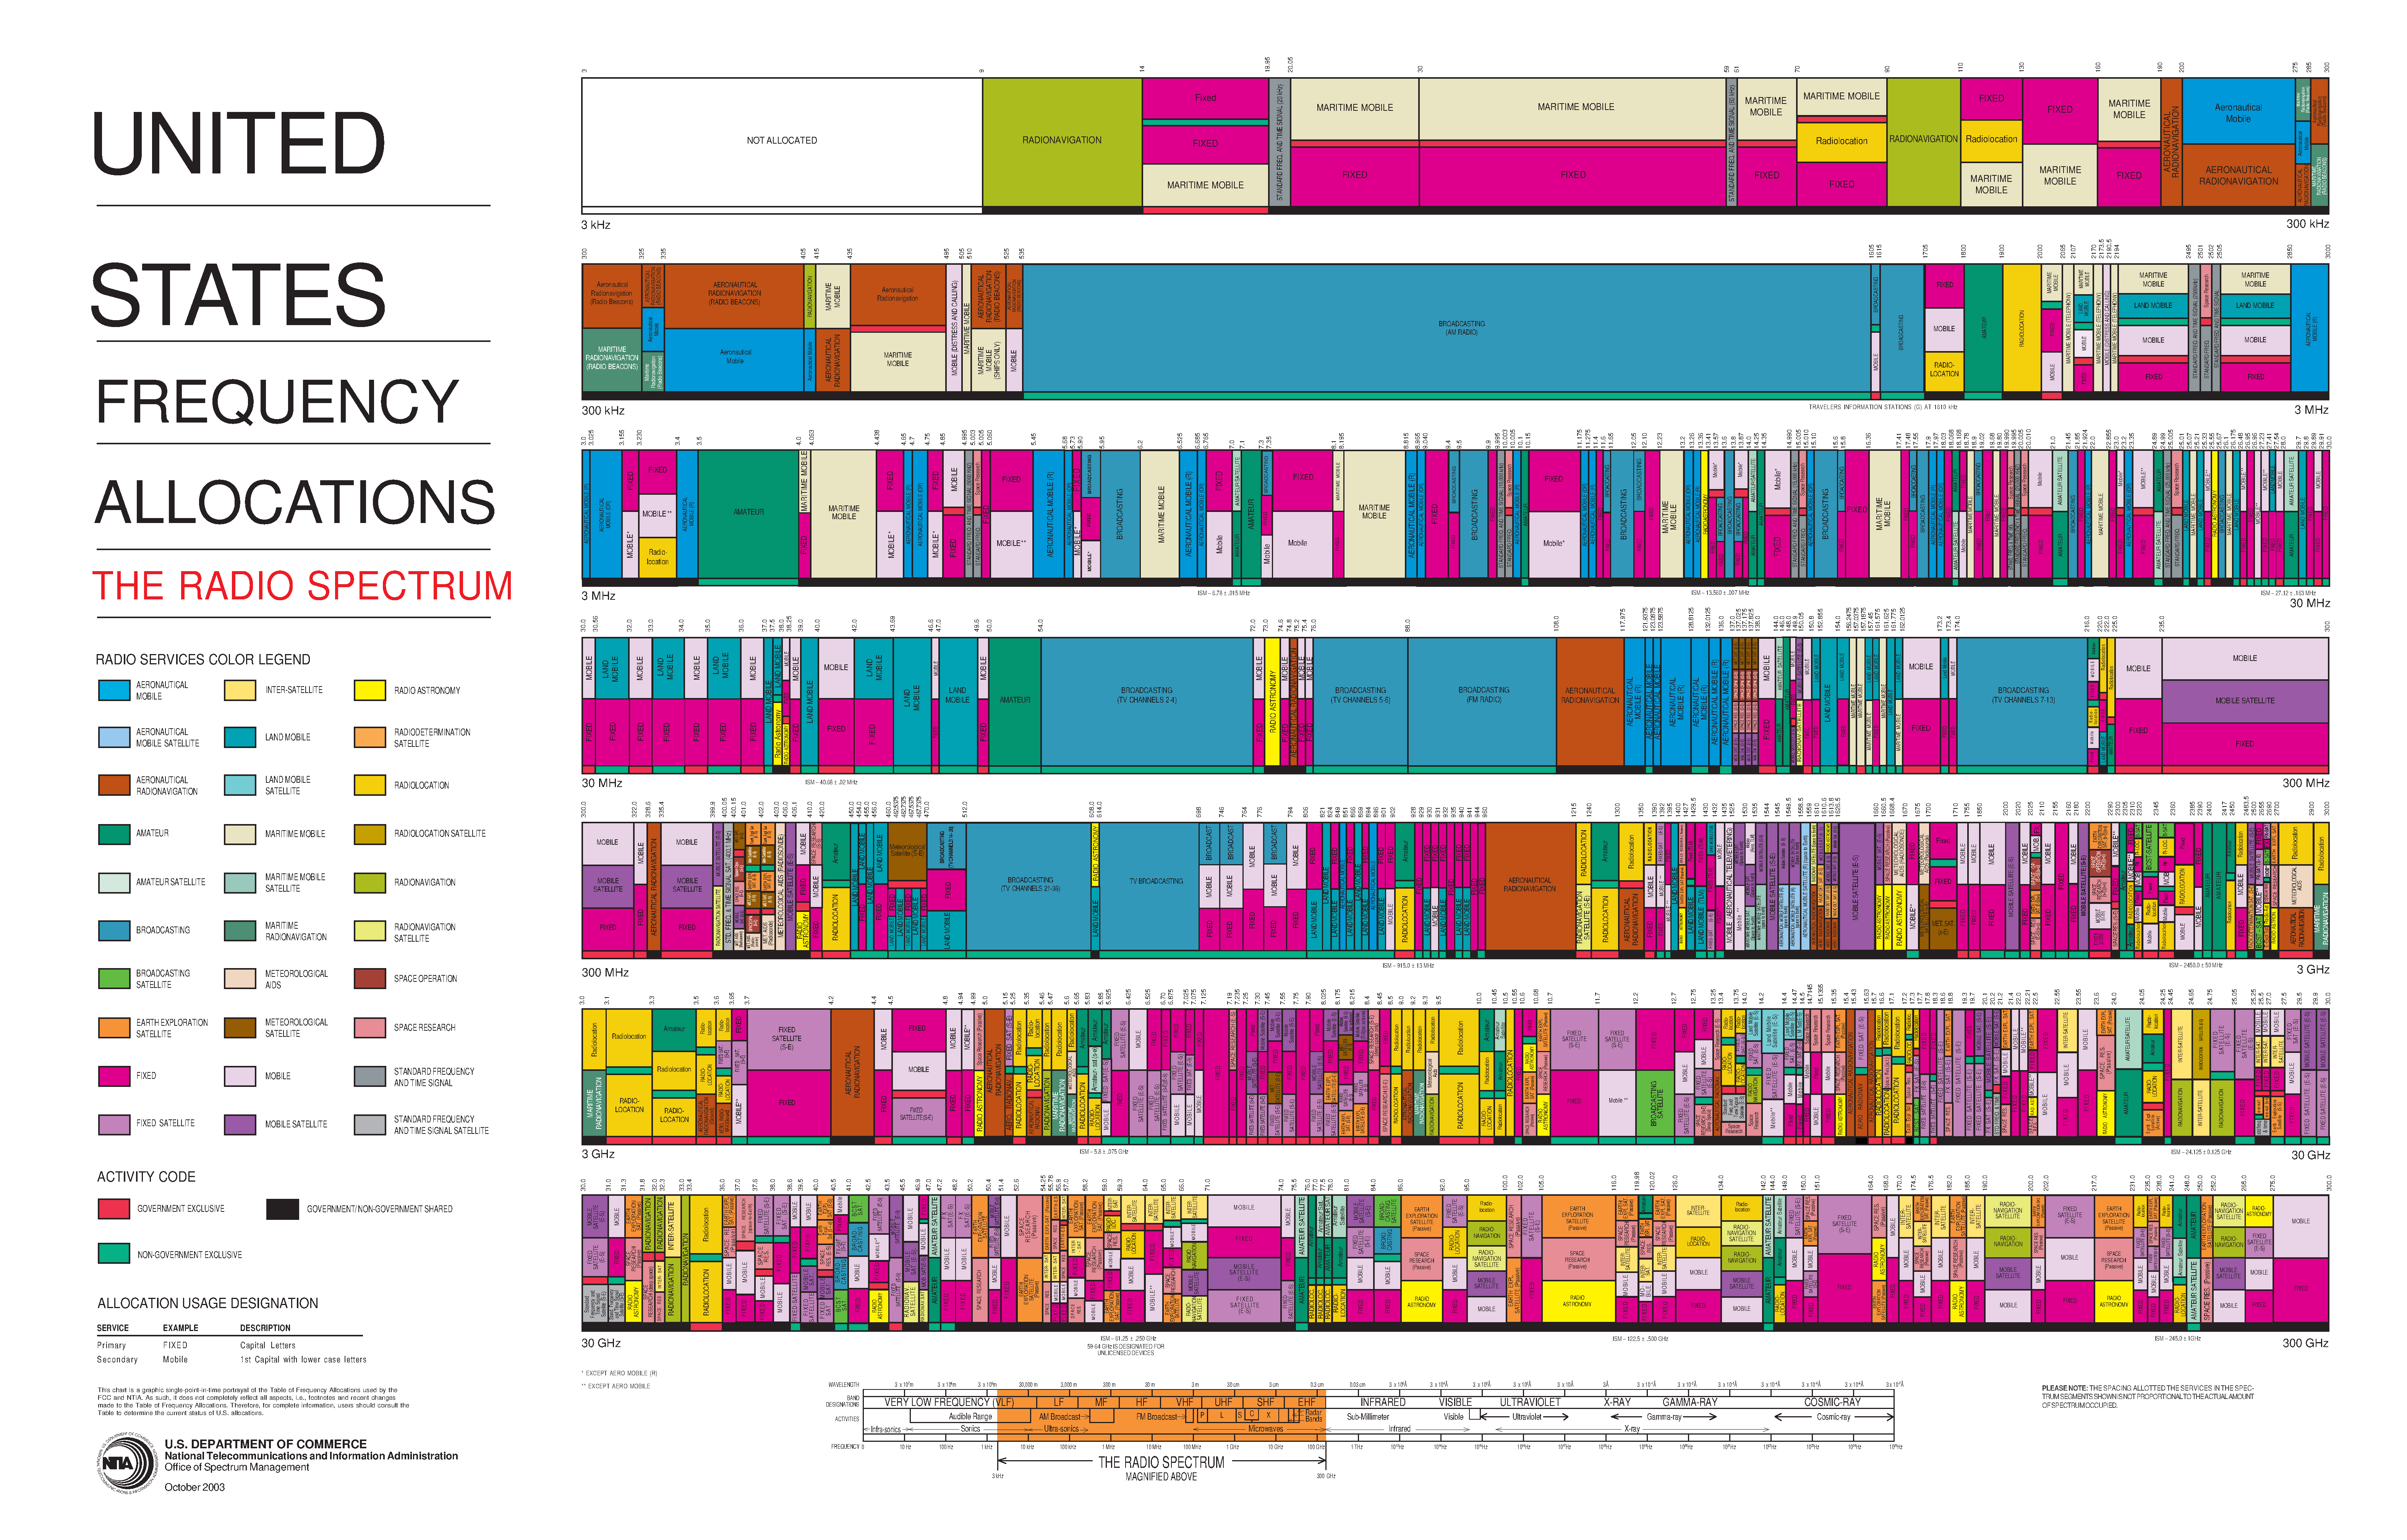
\includegraphics[width=\textwidth]{2003-allochrt.pdf}
\end{center}
\end{frame}

\section{Part 97}

\begin{frame}
\frametitle{47 CRF 97.1 Basic Purpose}
The rules and regulations in this part are designed to provide an amateur radio service having a fundamental purpose as expressed in the following principles:
\begin{enumerate}[A]
\scriptsize\item  Recognition and enhancement of the value of the amateur service to the public as a \emph{voluntary noncommercial communication service}, particularly with respect to providing emergency communications.\pause
\item Continuation and extension of the amateur's proven ability to contribute to the advancement of the radio art.\pause
\item Encouragement and improvement of the amateur service through rules which provide for advancing skills in both the communication and technical phases of the art.\pause
\item  Expansion of the existing reservoir within the amateur radio service of trained operators, technicians, and electronics experts. \pause
\item Continuation and extension of the amateur's unique ability to enhance international goodwill.
\end{enumerate}
\end{frame}

\begin{frame}
\frametitle{Key phrase}
\begin{alltt}
\ldots\emph{a voluntary noncommercial\\communications service}\ldots
\end{alltt}
This phrase sums up almost every rule and tenant of amateur radio.
\end{frame}

\begin{frame}
\frametitle{A voluntary noncommercial communications service}
Noncommercial means no ``pecuniary interest''. It is illegal to profit from the use of amateur radio.\\
\hfil \\As with almost any rule there are exceptions
\begin{itemize}
\item Teachers may use ham radio in the classroom as a teaching aid
\item ``Code practice'' transmissions
\item Disaster Drills
\end{itemize}
\end{frame}

\begin{frame}
\frametitle{More basic rules}
\begin{itemize}
\item No Music - expect transmission or re-transmission of a signal from a space station
\item No Broadcasting
\item No commercial traffic
\item No profanity
\item No codes or ciphers intended to hid content
\item No international third party traffic unless treaty-approved
\end{itemize}
\end{frame}

\section{Licenses}

\begin{frame}
\frametitle{Licenses}
A license is valid for ten years, with a two year grace period. Upgrades don't count as renewals. Basic renewals are free!\\
There are five classes.
\begin{itemize}
\item *Novice
\item Technician
\item General
\item *Advanced
\item Extra
\end{itemize}
\end{frame}

\begin{frame}
\frametitle{Licenses}
There are four kinds of licenses, Individual hams hold both a ``Station'' and ``Operator''
\begin{itemize}
\item Station
\item Operator
\item Club - W7OSU, K7CVO, W1AW
\item Special Event - A7W
\end{itemize}
Clubs can get a ``club callsign'', and events can get an event callsign.
\end{frame}

\section{Callsigns}

\begin{frame}
\frametitle{Callsigns}
\begin{itemize}
\item US callsigns start with A,K,N, or W
\item The format is one or two letters, a number, and one to three letters.
\item New callsigns are assigned in sequential order - number indicates the region in the US
\item Shorter callsigns are reserved for higher license classes
\item 1X1 for special events only
\end{itemize}
\end{frame}

\begin{frame}
\frametitle{Callsigns}
\begin{itemize}
\item KE7OSN
\item N8GFO -Yep\pause
\item K7HZ -That's an Extra\pause
\item VE6GLW -That's Canadian\pause
\item KLOO -That's a commercial station\pause
\item WSJ509 -Land Mobile, Benton County Sheriff\pause
\item Mission Base -What is known as a ``tactical callsign''\pause
\end{itemize}
\end{frame}

\begin{frame}
\frametitle{Operator}
Who ``operates'' an amateur station? \pause \\
The control operator, who is designated by the station licensee, and determines the privileges of operation.\\
e.g.\ if you are at a radio that can operate outside your privileges, you still can only use what you are licensed to.
\end{frame}

\begin{frame}
\frametitle{Your Callsign}
A station must transmit it's callsign at least every ten minutes and at the end of every communication.\\
Special situations have special rules\\
\begin{itemize}
\item Control operator working outside of a station licensee privileges.
\item Special event station control operator
\item Control operator using new privileges prior to FCC database update
\end{itemize}
\end{frame}

\begin{frame}
\frametitle{The Uniform Licensing System}
The ULS is an online database of FCC license information. A new licensee may use their privileges as soon as their information appears in the ULS. When you upgrade you may use your new privileges as soon as you pass the test.
\end{frame}

\begin{frame}
\frametitle{Typical uses of a callsign}
\begin{itemize}[<+->]
\item W7OSU This is KE7OSN
\item Net Control This is KE7OSN
\item This is W7OSU (Go Ahead)
\item CQ CQ CQ this is KE7OSN
\item KE7OSN monitoring
\item This is KF7FGE stroke (/) KE7OSN
\item Hey Bob, you around?
\end{itemize}
\end{frame}

\begin{frame}
\frametitle{Hey bob, you around}
Hey bob you around?\\
Legal? \\ \pause
Yes, as long as you keep to the every ten minutes and the end of every communication. \\ \pause
What if Bob isn't there? \\ \pause
KE7OSN clear
\end{frame}

\begin{frame}
\frametitle{Types of stations}
\begin{itemize}
\item Club – at least four  people, one of which accepts responsibility and is the “trustee”.
\item Space – at least 50km above the surface.
\item Beacon --  transmits a low-level signal for propagation studies
\item Repeater – re-transmits  a signal heard on one frequency on another frequency.
\item Auxiliary – a secondary receiver that feeds a repeater station.  
\end{itemize}
\end{frame}

\section{Frequencies}

\begin{frame}
\frametitle{Band Plan}
\begin{center}
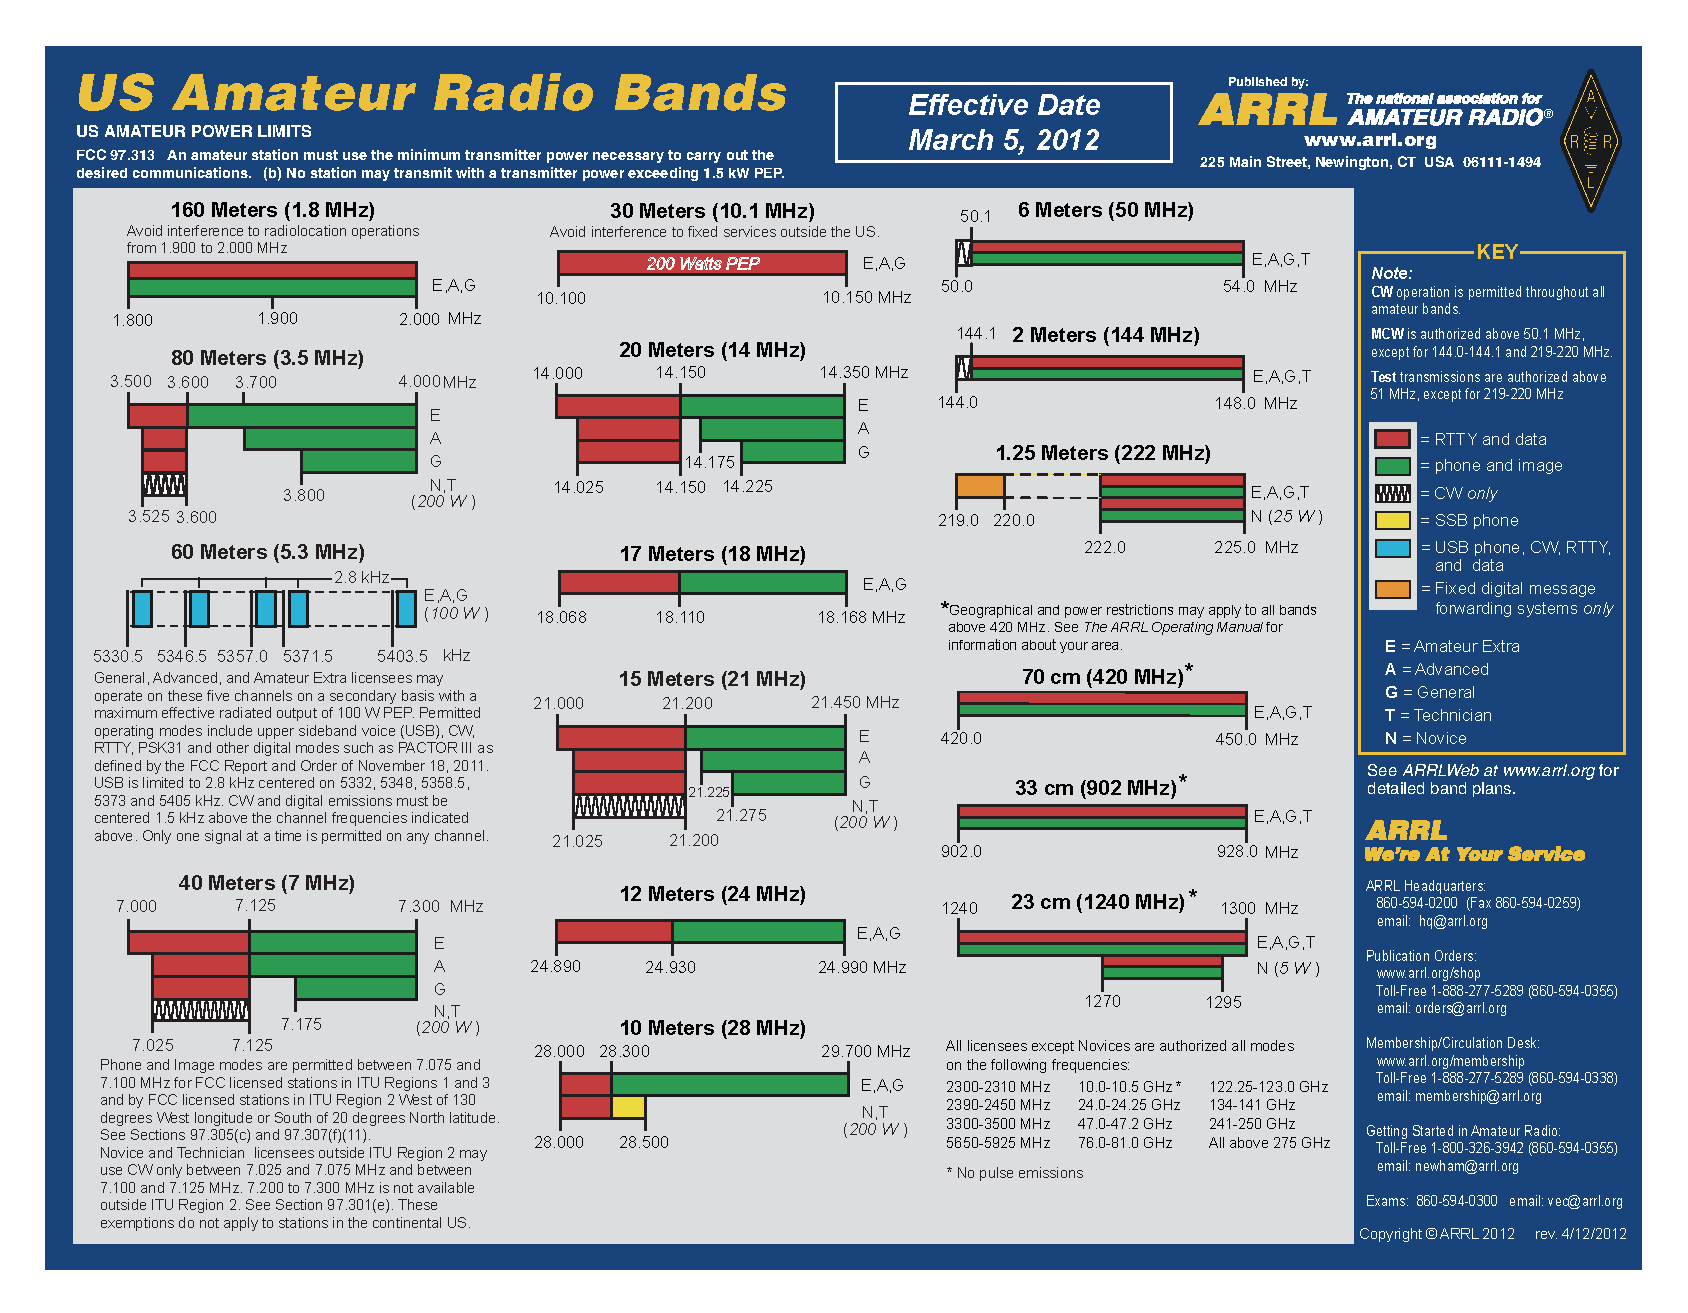
\includegraphics[height=.9\textheight]{hambandscolor.pdf}
\end{center}
\end{frame}

\begin{frame}
\frametitle{ITU Band Names}
\begin{itemize}
\item MF - Medium Frequency 300KHz to 3MHz
\item HF - High Frequency 3MHz to 30 MHz
\item VHF - Very High Frequency 30MHz to 300MHz
\item UHF - Ultra High Frequency 300MHz to 3GHz
\item SHF - Super High Frequency 3GHz to 30GHz
\item EFE - Extremely High Frequency - 30GHz to 300GHz
\item THF - Tremendously High Frequency - 300GHZ to 3THz
\end{itemize}
\end{frame}

\begin{frame}
\frametitle{HF 3-30MHz}
	\begin{itemize}
	\item 80 Meters
		\begin{itemize}
		\item 3.525-3.600MHz: CW Only
		\end{itemize}
	\item 40 Meters
		\begin{itemize}
		\item 7.025-7.125MHz: CW Only
		\end{itemize}
	\item 15 Meters
		\begin{itemize}
		\item 21.025-21.200MHz: CW Only
		\end{itemize}
	\item 10 Meters 
		\begin{itemize}
		\item  28.000-28.300MHz: CW, RTTY/Data 200 watts PEP max 
		\item 28.300-28.500MHz: CW, Phone 200 watts PEP max
		\end{itemize}
	\end{itemize}
\end{frame}

\begin{frame}
\frametitle{VHF 30-300MHz}
	\begin{itemize}
	\item 6 Meters
		\begin{itemize}
		\item 50.0-50.1MHz CW Only
		\item 50.1-54.0MHz All modes
		\end{itemize}
	\item 2 Meters
		\begin{itemize}
		\item  144.0-144.1MHz CW Only
		\item 144.1-148.0MHz All modes
		\end{itemize}
	\item 1.25 Meters
		\begin{itemize}
		\item 222.00-225.00MHz All modes
		\end{itemize}
	\end{itemize}
\end{frame}

\begin{frame}
\frametitle{UHF 300-3000MHz (3GHz)}
\begin{itemize}
\item 70 Centimeters
\begin{itemize}
\item 420.0-450.0MHz All Modes
\end{itemize}
\item 33 Centimeters
\begin{itemize}
\item 902.0-928.0MHz All Modes
\end{itemize}
\item 23 Centimeters
\begin{itemize}
\item 1240-1300MHz All Modes
\end{itemize}
\item 2.4GHz
\begin{itemize}
\item 2.3-2.31GHz
\item 2.39-2.45GHz *
\end{itemize}
\end{itemize}
\end{frame}

\begin{frame}
\frametitle{2.4GHz}
We share the 2390-2450MHz band with: 802.11 networks, cordless phones, video cameras, zigbee, etc.\ \\
We are PRIMARY users. We have first ``rights''. Secondary users must not cause us interference and must accept interference from our operations.
\end{frame}

\begin{frame}
\frametitle{SHF 3GHz-30GHz and up}
\begin{itemize}
\item 3.3-3.5GHz
\item  5.65-5.925GHz
\item  10.0-10.5GHz
\item  24.0-24.25GHz
\item  47.0-47.2GHz
\item  76.0-81.9GHz
\item  119.98-120.02GHz
\item  142-149GHz
\item  241-250GHz
\item  Everything above 300GHz
\end{itemize}
\end{frame}

\part{Station operation; choosing an operating frequency, calling another station, test transmissions, use of minimum power, frequency use, band plans}

\section{Emergency Operations}
\begin{frame}
\frametitle{97.403 Safety of life and protection of property}
No provision of these rules prevents the use by an amateur station of any means of radio communication at its disposal to provide essential communication needs in connection with the immediate safety of human life and immediate protection of property \textbf<2->{when normal communication systems are not available.}
\end{frame}

\begin{frame}
\frametitle{ARES}
ARES – \textbf{A}mateur \textbf{R}adio \textbf{E}mergency \textbf{S}ervice
\begin{itemize}
\item Organized and run by ARRL
\item Supports governmental and NGO groups.
\item Most groups are organized at the county level
\item “EC” – Emergency Coordinator
\end{itemize}
\end{frame}

\begin{frame}
\frametitle{RACES}
RACES – \textbf{R}adio \textbf{A}mateur \textbf{C}ivil \textbf{E}mergency \textbf{S}ervice
\begin{itemize}
\item Defined by the FCC
\item Supports governmental agencies ONLY.
\item Operators are registered with the controlling agency. 
\item RACES Officer
\item Activated by federal declaration of emergency. 
\item In Oregon, ARES members are also registered in RACES
\end{itemize}
\end{frame}

\section{Nets and messages}
\begin{frame}
\frametitle{Disaster == Organized Chaos}
To keep some organization to the use of frequencies and communications,  groups are organized into “nets”.

A “net” is a group of stations that are cooperating in the use of a frequency. The “net control” is responsible for deciding who gets to talk. 
\end{frame}

\begin{frame}
\frametitle{Disaster == Organized Chaos}
There are two kinds of nets:
 \begin{description}
\item[Directed] - the net control is strict in controlling who talks to whom.  Stations tell net control they have a message for another station, and the net control directs them to call that station and pass the message.
\item[Free] - the net control allows stations to contact each other as they need to.   
\end{description}
\end{frame}

\begin{frame}
\frametitle{Disaster == Organized Chaos}
There are three types of messages
\begin{description}
\item[Formal] - written messages.
\item[Informal] - unwritten messages.
\item[Administrative] - station to station housekeeping.
\end{description}
\end{frame}

\begin{frame}
\frametitle{Written Messages – Formal Traffic}
ARES and RACES have adopted the NIMS/ICS system for written traffic. I.e., ICS-213 message forms, in either digital or transcribed versions.\\ \hfil \\
 
\uncover<2->{The TEST doesn't ask you about that. The TEST deals with the National Traffic System message form.}
\end{frame}

\begin{frame}
\frametitle{Written Messages – Formal Traffic}
The National Traffic System (NTS) is a system organized by ARRL to transmit messages in a standard format, usually concerning “Health and Welfare”. For example: “Aunt Martha arrived home safely. Have a happy birthday.”  Or “welcome to Ham radio”. \\

These messages use the NTS RadioGram form. The process is described in depth in the Message Processing Guidelines (MPG).
\end{frame}

\begin{frame}
\frametitle{NTS RadioGram Form}
\centering 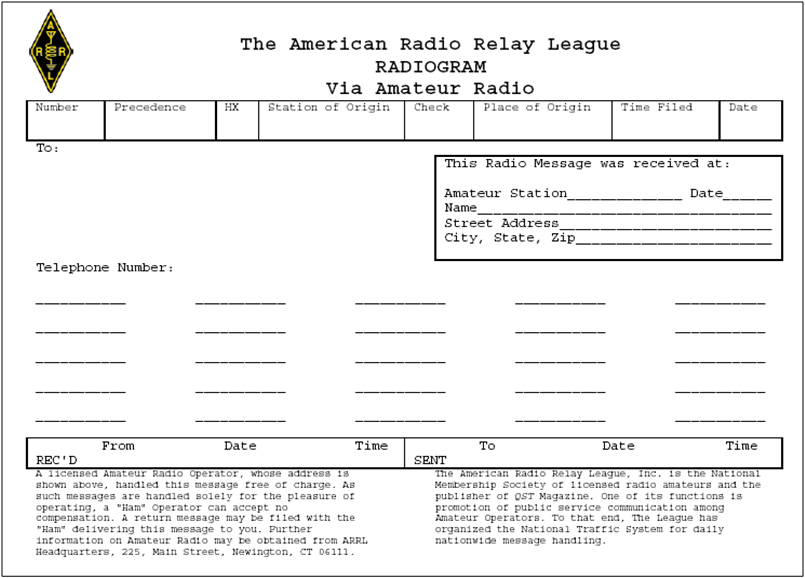
\includegraphics[width=\textwidth]{radiogramform.png}
\end{frame}

\section{Radio Speak}
\begin{frame}
\frametitle{Types of radio short-hand}
Amateur radio has its own codes, and slang. Much like 1337 or txt, this ``shared language'' makes it easier to communicate quickly, and efficiently. Much of it comes from the days of telegraph and Morse Code.
\begin{description}
\item[Q Codes] - Three letter codes beginning with Q
\item[Number codes] - Codes sent as numbers, we really only us 73
\item[Pro-words] - Standardized ways of saying things in a clear and concise fashion
\item[Phonetics] - Words for letters, try saying BCDEZGT five times fast.
\end{description}
\end{frame}

\begin{frame}
\frametitle{Q-Codes}
Q codes are three letter codes that begin with Q and not QU and can be sent as either a question or a response. Really useful when using Morse Code as the codes are much shorter than what they represent. Some common Q codes are listed below.
\begin{description}
\item[QSY] Change frequency
\item[QRT] Stop transmitting
\item[QRZ] I'm calling
\item[QR\textbf<2->{M}] \textbf<2->{M}an made interference
\item[QR\textbf<2->{N}] \textbf<2->{N}atural interference or \textbf<2->{N}oise
\item[QSL] Acknowledge
\item[QST] Message to all amateurs
\end{description}
\end{frame}

\begin{frame}
\frametitle{Pro-words}
Pro or Professional words are used as shorthand, and because they prevent confusion. Yea and Nah kinda sound the same.
\begin{description}
\item[Roger] Received
\item[WilCO] Will Comply
\item[Over] I'm done talking for now
\item[Out] I'm done talking to you
\item[This Is] I'm going to say my callsign now
\item[Wait] Hold on for a while
\item[Affirmative] Yes
\item[Negative] No
\end{description}
\end{frame}

\begin{frame}
\frametitle{Phonetics}
In amateur radio we use ITU phonetics, this helps us reduce the potential of confusion over letters that sound the same
\begin{tabular}{l l l}
\scriptsize A - Alfa ``AL-FAH''& \scriptsize  N - November ``NO-VEM-BER'' & \scriptsize  0 ``ZEE-RO''\\
\scriptsize B - Bravo ``BRAH-VOH''& \scriptsize  O - Oscar ``OSS-CAH'' & \scriptsize  1 ``WUN''\\
\scriptsize C - Charlie ``CHAR-LEE''& \scriptsize  P - Papa ``PAH-PAH'' & \scriptsize  2 ``TOO''\\
\scriptsize D - Delta ``DELL-TAH''& \scriptsize  Q - Quebec ``KEH-BECK'' & \scriptsize  3 ``TH-UH-REE''\\
\scriptsize E - Echo ``ECK-OH''& \scriptsize  R - Romeo ``ROW-ME-OH'' & \scriptsize  4 ``FOW-ER''\\
\scriptsize F - Foxtrot ``FOKS-TROT''& \scriptsize  S - Sierra ``SEE-AIR-RAH'' & \scriptsize  5 ``FI-IV'' OR ``FIFE''\\
\scriptsize G - Golf ``GOLF''& \scriptsize  T - Tango ``TANG-GO'' & \scriptsize  6 ``SIX''\\
\scriptsize H - Hotel ``HOH-TELL''& \scriptsize  U - Uniform ``YOU-NEE-FORM'' & \scriptsize  7 ``SEV-EN''\\
\scriptsize I - India ``IN-DEE-AH''& \scriptsize  V - Victor ``VIK-TAH'' & \scriptsize  8 ``ATE''\\
\scriptsize J - Juliet ``JEW-LEE-ETT''& \scriptsize  W - Whiskey ``WISS-KEY'' & \scriptsize  9 ``NIN-ER''\\
\scriptsize K - Kilo ``KEE-LOH''& \scriptsize  X - X-Ray ``ECKS-RAY''\\
\scriptsize L - Lima ``LEE-MAH''& \scriptsize  Y - Yankee ``YANG-KEY''\\
\scriptsize M - Mike ``MIKE''& \scriptsize  Z - Zulu ``ZOO-LOO''\\
\end{tabular}
W7QH becomes ``Whiskey 7 Quebec Hotel'' 
\end{frame}

\begin{frame}
\frametitle{CQ and 73}
There are two other special cases.
\begin{itemize}
\item CQ is the standard calling call. Think of it as Seek You, though no one really knows where it comes from. It is common to add extra stuff depending on the situation. You might hear CQ JOTA, CQ Field Day, CQ Contest, CQ DX, CQ Oregon. This lets people pick who they are looking for. A common general CQ would sound like ``CQ CQ CQ this is KE7OSN calling CQ CQ CQ''
\item The other thing that comes up is the number 73, this goes back to the old Western Union Telegraph 92 codes, these were numbers that could be used in place of certain phrases, most of them dealing with packages or trains. 73 means ``Beast Regards'' and is generally used as ``goodbye''
\end{itemize}
\end{frame}

\section{Other Practices}

\begin{frame}
\frametitle{Power}
In most amateur bands the maximum legal limit for power output is 1500 Watts, PEP. PEP - Peak Envelope Power is the largest amplitude of a signal. On some bands the limit is lower, for each band there is also a point at which you have to do a safety evaluation of your station to avoid unsafe exposure. You should always use the minimal power required to do what you need to do.
\end{frame}

\part{Radio wave characteristics, radio and electromagnetic properties, propagation modes}
\section{Electromagnetic Waves}
\begin{frame}
\frametitle{Electromagnetic Waves}
Electromagnetic waves are energy waves that move through space, similar to the way waves move in water or sound through air.\\
In a vacuum these waves move at the speed of light 299,792,458$m/s$ or 186,282.397$miles/second$. This is good as these waves are light.
\end{frame}

\begin{frame}
\frametitle{Speed of light}
We can round up to 300,000,000$m/s$. Some distance measured in terms of light-time
\begin{description}
\item[Average distance between the Sun and Earth] - 8 minutes
\item[GEO Satellite to Earth's Surface] - about a half second
\item[Nearest other star to our Sun] 4.25 Years
\item[Voyager Space probe to the Sun] at 18,884,401,200 Km from the sun? \only<2->{$\frac{\frac{18884401200Km}{300000Km/s}}{3600s}=Hours$} \only<3->{17:08:00-ish}
\end{description}
\end{frame}

\begin{frame}
\frametitle{Frequency - not just an ok movie}
We often refer to a wave by it's frequency. Frequency is the number of times a wave cycles in a given time. We use Hertz (Hz) which has the unites of $\frac{1}{Seconds}$.\\
Middle C is 440Hz, or 440 cycles per second.\\
KLOO-AM is 1.340MHz, or 1,340,000 cycles per second.
\end{frame}

\begin{frame}
\frametitle{SI Prefixes}
Sometimes it is a lot easier to shorten things up a bit.
\begin{description}
\item[Tera]T $10^{12}$ 1,000,000,000,000
\item[Giga]G $10^9$ 1,000,000,000
\item[Mega]M $10^6$ 1,000,000
\item[Kilo]K $10^3$ 1,000
\item[Deci]d $10^{-1}$ 0.1
\item[Ceni]c $10^{-2}$ 0.01
\item[Milli]m $10^{-3}$ 0.001
\item[Micro]$\mu$ $10^{-6}$ 0.000001
\item[Nano]n $10^{-9}$ 0.000000001
\item[Pico]p $10^{-12}$ 0.000000000001
\end{description}
\end{frame}

\begin{frame}
\frametitle{Wavelength}
We also use wavelength to describe waves. The wavelength is the distance between two like points on the wave exactly one cycle apart, e.g.\ the distance between peaks.\\
\begin{center}
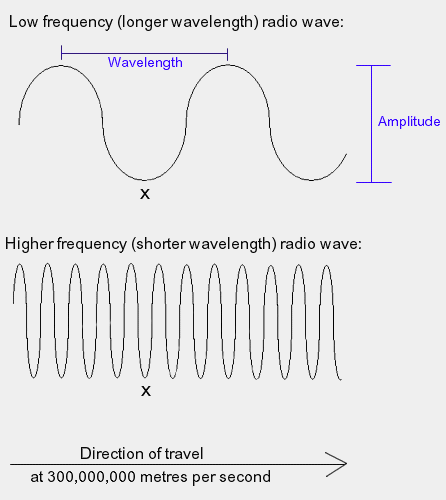
\includegraphics[width=0.85\textwidth,height=0.7\textheight]{wavelength.png}
\end{center}
\end{frame}

\begin{frame}
\frametitle{Electromagnetic}
\begin{center}
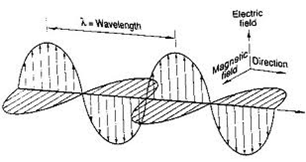
\includegraphics[height=0.5\textheight]{emwave.png}\\
\end{center}
Electromagnetic waves have two parts, one electric part, and one magnetic part. The magnetic part is rotated and phase shifted by 90$^{\circ}$
\end{frame}

\begin{frame}
\frametitle{Wavelength to frequency and back}
It is easy to convert between wavelength and frequency just use the equation below.\\
\only<2->{$Wavelength(meters) = \frac{300}{Freq. (MHz)}$\\}
\only<3->{We'll practice on the next slide}
\end{frame}

\begin{frame}
\frametitle{MATH!!!}
\begin{itemize}
\item Lets try to convert 7.025MHz into a wavelength to figure out which band it belongs to.\\
\only<2->{$Wavelength(\lambda)=\frac{300}{7.025}$} \only<3->{that comes out to 42.7meters\\}
\only<4->{That fits nicely in the 40meter band\\}
\item<5-> Now lets try 223.50MHz\\
$\frac{300}{223.50}=?$ \only<6->{1.35, for the 1.25meter band.}
\end{itemize}
\end{frame}

\section{Propagation}
\begin{frame}
\frametitle{Line of sight}
Just like light radio waves travel in a straight line.\\
\only<2->{They also reflect off some things like light.\\}
\only<3->{If there are multiple ways for radio waves to get between two points we call this Multipath, and it creates interference.\\}
\only<4->{Reflections can be really useful when you don't have a direct line of sight.\\}
\only<5->{Radio waves will also refract.\\}
\end{frame}

\begin{frame}
\frametitle{Solar Wind}
\begin{center}
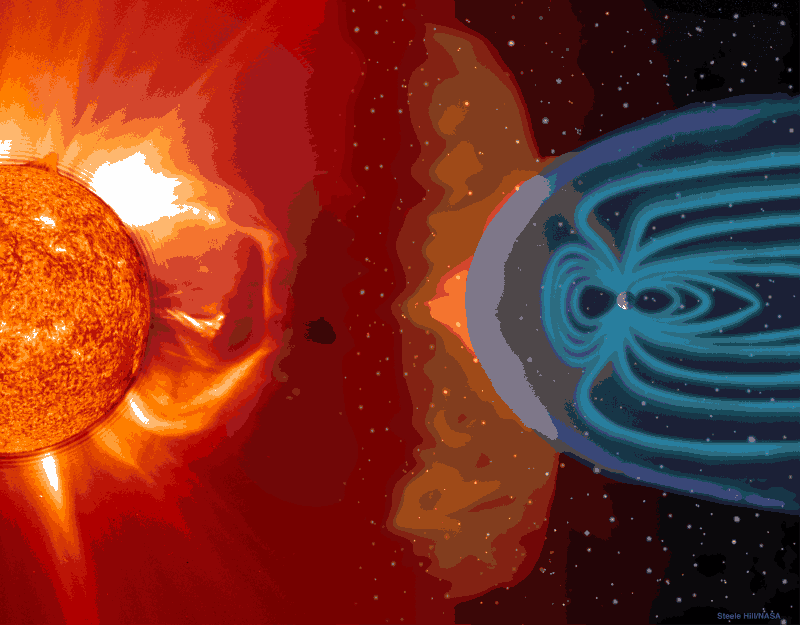
\includegraphics[width=\textwidth]{magfield.png}
\end{center}
\end{frame}

\begin{frame}
\frametitle{Solar Radiation}
Solar radiation charges atoms in the atmosphere, breaking loose electrons, to create ions, which can interact with radio waves.\\
\begin{columns}
\column{.3\textwidth}
At night the electrons recombined with their atoms. This means things change from day to night.
\column{.7\textwidth}
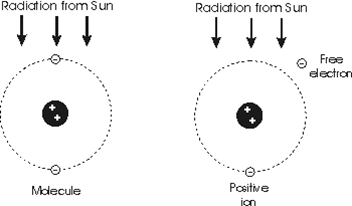
\includegraphics[width=\textwidth]{ions.png}
\end{columns}
\end{frame}

\begin{frame}
\frametitle{Ionosphere}
\begin{columns}
\column{.6\textwidth}
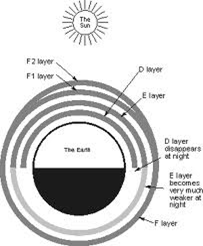
\includegraphics[height=.9\textheight]{ionosphere.png}
\column{.4\textwidth}
The parts of the atmosphere most affected by ionization are collectively called the Ionosphere!\\
It has multiple layers, each interact differently with radio waves. The D layers mostly absorbs RF, while the E and F layers reflect.\\
HF is is ruled by the ionosphere\\ VHF and up \ldots not so much.
\end{columns}
\end{frame}

\begin{frame}
\frametitle{Ionosphere}
During the day the D layers absorbs a large chunk of HF, at night it goes away and signals bounce (refract) off the E and F layers.\\
VHF and above mostly just goes through the ionosphere\ldots\\
But sometimes at night there is just enough E layer to refract VHF signals. We call this ``Sporadic E''
\end{frame}

\begin{frame}
\frametitle{Auroras and Meteor Showers}
The auroras are a visible sign of ionization, as they move they can cause received signals to sound fluttery.\\
Meteor showers leave short lived trails of ionized gases, that can refract signals, these effects are impossible to predict and last seconds.\\
You can even bounce radio signals off the moon!
\end{frame}

\begin{frame}
\frametitle{Tropospheric Ducting}
\begin{center}
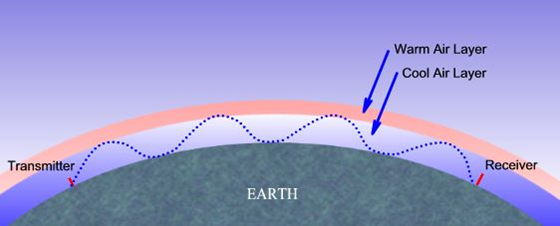
\includegraphics[width=\textwidth]{troposhpere.png}
\end{center}
Air can refract electromagnetic radiation. A temperature inversion (warm air above cold) can cause VHF signals to refract and travel long distances.\\
This is called ``Tropospheric Ducting'' and often happens between here and Hawaii, it mostly affects VHF.
\end{frame}

\begin{frame}
\frametitle{Knife Edge}
\begin{center}
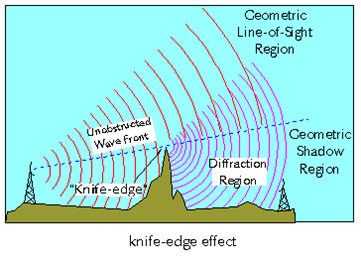
\includegraphics[height=.9\textheight]{knifeedge.png}
\end{center}
\end{frame}

\begin{frame}
\frametitle{Polarization}
Antennas tend to radiate and receive waves polarized along the direction of the antenna. An antenna pointing vertically produces vertically polarized waves, and the equivalent is true for a horizontal antenna.\\
If the polarization of the receiving antenna does not match the wave it is receiving then the signal strength is reduced by a significant degree. In an ideal world without the magnetic portion of a wave two antennas rotated $\pm90^{\circ}$ would not be able to ``see'' each other.
\end{frame}

\part{Amateur radio practices and station set up}
\begin{frame}
\frametitle{Technician class section 4}
This section is going to be really short as much of the details fit in better elsewhere
\end{frame}
\section{Station setup; microphone, speaker, headphones, filters, power source, connecting a computer, RF grounding}
\begin{frame}
\frametitle{Station setup; microphone, speaker, headphones, filters, power source, connecting a computer, RF grounding}
Some microphones include push-to-talk and voltage connections. Headphones can be useful in a noisy area instead of a speaker. A regulated power supply reduces voltage fluctuations. Filters between the transmitter and antenna can reduce harmonic emissions. A band-reject filter is a good first step if your 2 meter radio is causing problems with a TV. A terminal node controller is a modem for your radio, your sound card can be a modem too. Flat straps are good grounding cables. Ferrite chokes can reduce RF current in cables. If your radio whines in your car and it goes along with the engine its probably the alternator. A radio installed in a car should be connected to a good ``ground''
\end{frame}

\section{Operating controls; tuning, use of filters, squelch, AGC, repeater offset, memory channels}
\begin{frame}
\frametitle{Operating controls; tuning, use of filters, squelch, AGC, repeater offset, memory channels}
If your mic is turned up to loud your signal may distort. You can set the frequency of a radio with the keypad or VFO knob. Squelch lets you mute the receiver when no signal is coming in. You can program favorite frequencies in memory. The noise blanker option can reduce noise. The RIT or Receiver Incremental Tuning control can change the pitch of the received audio. A good filter setting for SSB is 2400Hz, and 500Hz for CW. A repeater offset is the difference in its receive and transmit frequencies.
\end{frame}

\part{Electrical principles, math for electronics, electronic principles, Ohm s Law}
\section{Ohm's Law}
\begin{frame}
\frametitle{Ohm, Ohm on the range}
Most metals are good at conducting electricity, this means they allow electrons to move around. We make wires that allow us to move electrons from one specific place to another.
\end{frame}
\subsection{Current}
\begin{frame}
\frametitle{Current}
The movement of electrons is called \textbf{Current}. We measure current in the Ampere, aka the Amp, aka A (or I).\\
Current that moves in only one direction is called \textbf{Direct Current (DC)}. Current that changes direction regularly is called \textbf{Alternating Current (AC)}.\\
A device that measures current is an ammeter.
\end{frame}

\begin{frame}
\frametitle{Ideas of current}
\begin{center}

\includegraphics[height=.9\textheight]{acdc.jpg}<1>
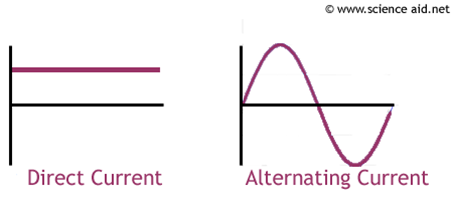
\includegraphics[width=\textwidth]{acdc.png}<2>
\end{center}
\end{frame}

\subsection{Voltage}
\begin{frame}
\frametitle{The Electromotive Force}
The force that causes electrons to flow is called \only{\ldots}<1>\pause \textbf{The Electromotive Force}.\\
 We measure this force as \only{\ldots}<2>\pause\textbf{ Voltage}, or \textbf{V}.\\
Voltage is measured with a \only{\ldots}<3>\pause \textbf{Voltmeter}
\end{frame}

\begin{frame}
\frametitle{Voltage}
Electrons like to spread out. It's their ``natural desire'' to not get bunched up that causes voltage. There can be voltage without current, but not current without voltage.\\
An unconnected battery has a voltage, but until it is hooked up to a complete circuit the electrons can't go anywhere.\\
Voltage is the difference in electrical potential between two points. Think of something falling down stairs.
\end{frame}

\subsection{Resistance}

\begin{frame}
\frametitle{The Resistor}
Resistance, impedes the flow of electrons.\\
The unit of resistance is the Ohm, or $\Omega$. \pause If that looks Greek, that's because it is, that Omega, a letter from the Greek alphabet\\ \only<3>{Now sing along \ldots \\ Alpha $A$, Beta $B$, Gamma $\Gamma$, Delta $\Delta$, Epsilon $E$, Zeta $Z$, Eta $H$, Theta $\Theta$, Iota $I$. \\Anyone? } \only{Resistance is measured with an ohmmeter.\\ Never use an ohmmeter on a live circuit}<4->
\begin{center}
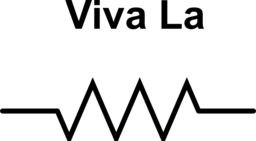
\includegraphics[width=.25\textwidth]{viva.png}<4->
\end{center}
\end{frame}

\subsection{Ohms Law}
\begin{frame}
\frametitle{Ohms Law}
The voltage across a resistor is equal to the resistance times the current. $V=IR$.\\
If we take a 9volt battery and connect it to a 90$\Omega$ resistor, what is the current through it?\pause\\
$V=IR\to I=\frac{V}{R}\to I=\frac{9}{90}$\pause$\to 0.1=\frac{9}{90}$ 0.1 Amps, or 100 milliamp.
\end{frame}

\begin{frame}
\frametitle{Power}
When current flows through an impedance it dissipates energy as ``POWER''. Power is measured Watts (W).\\
The equation for power is $P=IV$\pause Lets try with our prior example, we had 9volts and .1amps.\\
$P=IV \to P=9*.1$\pause$\to 0.9=9*.1$
\end{frame}

\section{Components}
\begin{frame}
\frametitle{Electrical Components}
\begin{center}
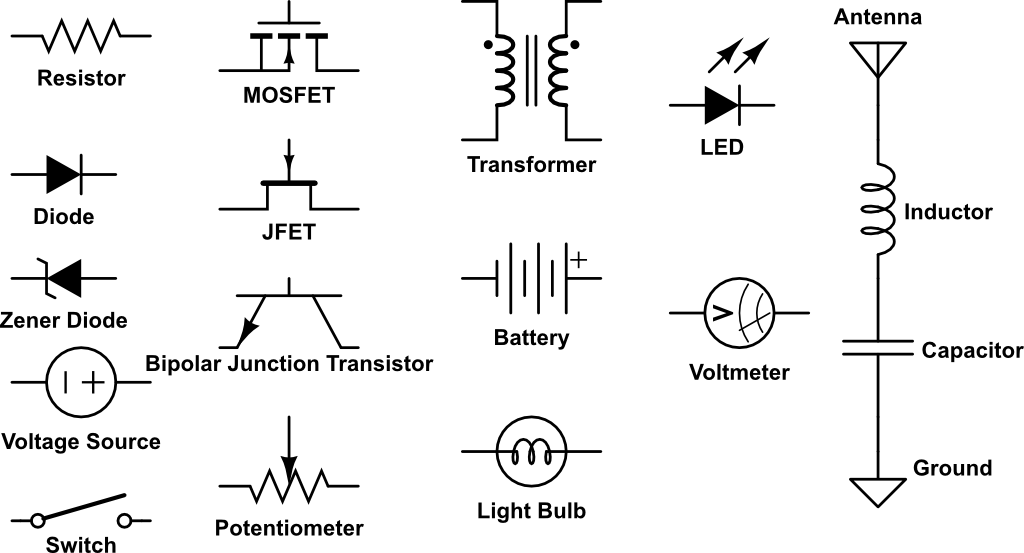
\includegraphics[width=\textwidth]{components.png}
\end{center}
\end{frame}

\subsection{The Resistor}
\begin{frame}
\frametitle{The Resistor}
Resistors are the electrical component that provides resistance. On paper they are squiggly lines, in real life they look like.\\\pause
\begin{center}
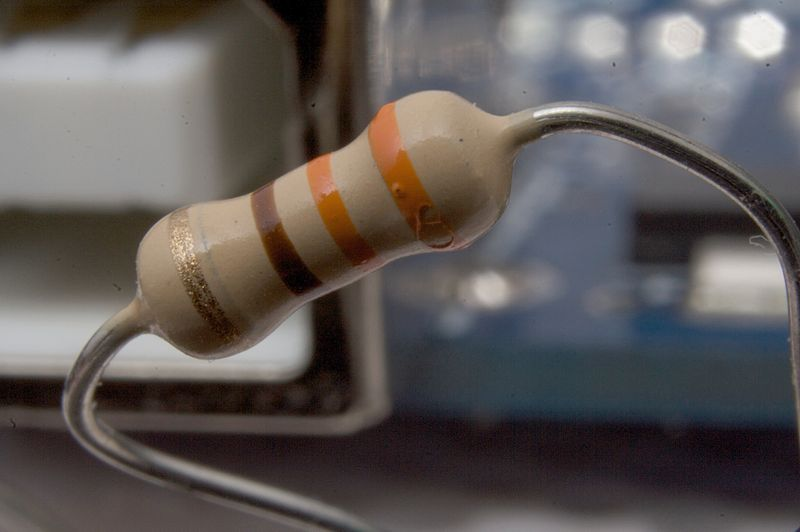
\includegraphics[height=.8\textheight]{resistor.jpg}
\end{center}
\end{frame}

\subsection{The Capacitor}
\begin{frame}
\frametitle{The Capacitor}
Capacitors store energy in an electrostatic field. They are made of two conducting plates separated by an insulated material. Electrons build up on one plate when charged. They pass AC fairly well, but can block DC. They are represented as two parallel lines, one may be curved. There are three types, a normal type that can be reversed, an electrolytic type that is polarized (they have a + or a - to note which way the go), and variable ones with an arrow through them.\\\pause
\begin{center}
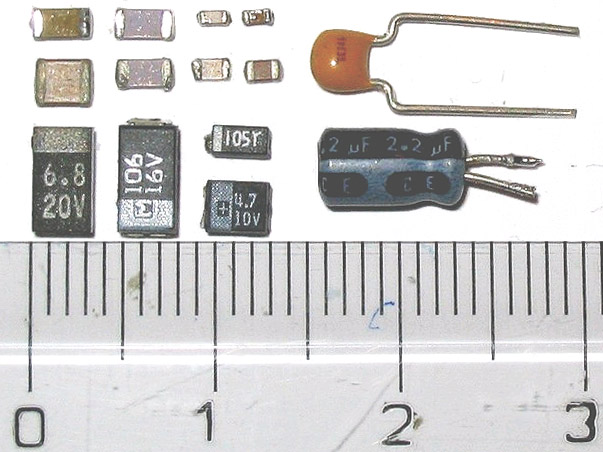
\includegraphics[height=.5\textheight]{capacitor.jpg}
\end{center}
\end{frame}

\begin{frame}
\frametitle{Warning}
\begin{center}
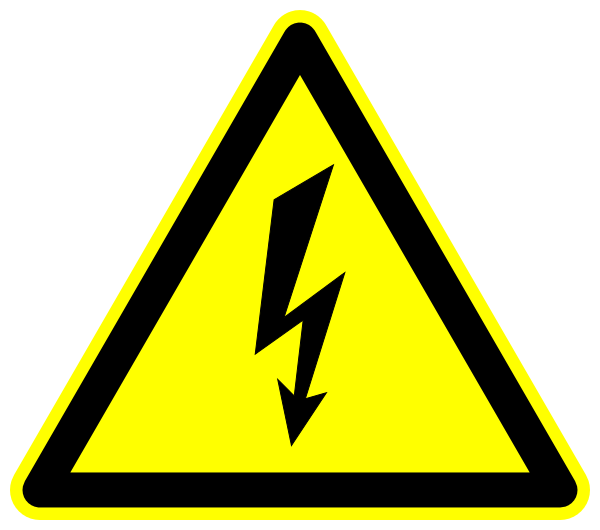
\includegraphics[height=.5\textheight]{shockhazard.png}
\end{center}
Capacitors can store a charge for some time. They can shock with ease, at best it will hurt, at worst it can cause burns and even stop your heart.
\end{frame}

\subsection{The Inductor}

\begin{frame}
\frametitle{The Inductor}
Inductors pass current in DC circuits, and impedes AC. They store energy in a magnetic field, magnetic fields require energy to change. This means that \textbf{any} change in current. The unit of inductance is the Henry.\\
They are made by winding wire in a coil. The more winds the more inductance. Sometimes iron is inserted in the middle to increase the inductance.
\begin{center}
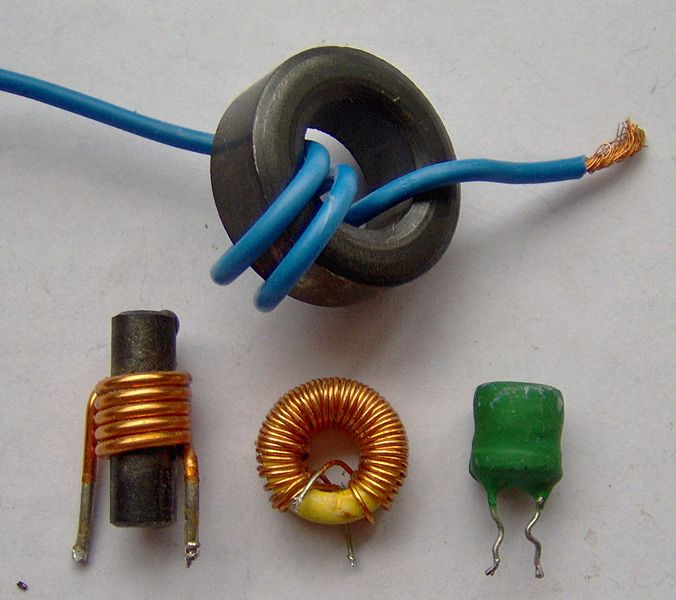
\includegraphics[height=.4\textheight]{inductor.jpg}
\end{center}

\end{frame}

\begin{frame}
\frametitle{More Inductance}
\begin{center}
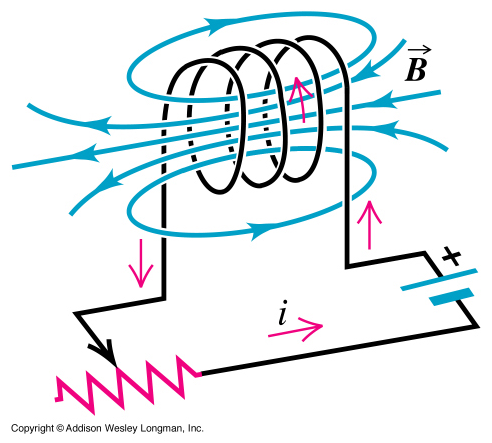
\includegraphics[height=.9\textheight]{inductor.png}
\end{center}
\end{frame}

\subsection{Relay}
\begin{frame}
\frametitle{Relays}
An inductor next to a magnetic switch creates a relay. They can be used to separate high current, or voltage circuits from low ones.
\end{frame}

\subsection{Diode}
\begin{frame}
\frametitle{Diodes}
Diodes prevent current from moving in one direction, while doing not much to current in the other. Some of them give off light. Others known as Zener diodes will let current flow against them if the voltage is high enough.\\
\begin{center}
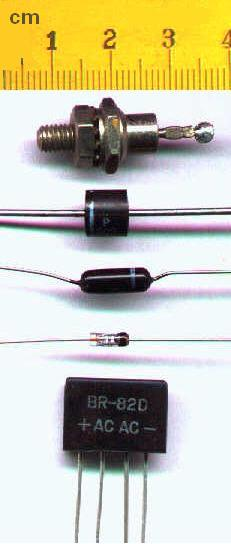
\includegraphics[angle=90,width=\textwidth]{diode.jpg}
\end{center}
\end{frame}

\subsection{Transistors}
\begin{frame}
\frametitle{Transistors}
Transistors allow a small current to control a much larger one. This gives transistors ``gain''. Two types we care about are Bi-polar Junction (BJT), and Field Effect (FET).
\end{frame}

\begin{frame}
\frametitle{BJT's}
Bipolar Junction Transistors come in two types, NPN and PNP. Both have three connections, an emitter, a collector, and a base. In diagrams the emitter is the wire with an arrow, the collector is on the same ``side'' as the emitter, and the base goes out the other way, if you turn it so it would stand on the two legs the base is the top. With an NPN current is allowed to flow from the collector to the emitter when there is enough voltage between the emitter and the base. In NPN's the arrow \textbf{N}ever \textbf{P}oints i\textbf{N}.\\PNP's allow current to flow from the emitter to the collector when there is enough voltage between the emitter and the base. For PNP's the arrow \textbf{P}oints i\textbf{N} \textbf{P}ermanently\\
\begin{center}
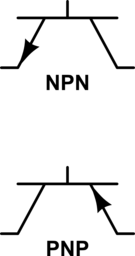
\includegraphics{bjts.png}
\end{center}
\end{frame}

\begin{frame}
\frametitle{MOSFET's}
Metal Oxide Semiconductor Field Effect Transistors work much like BJT's but they are a little different. In the diagrams if the arrow points out they are P-channel, and if it points i\textbf{N} its an N-channel. The three wires are a Gate, a Drain, and a Source. The wire with the arrow is the source, the drain is on the same side as the source, and the other one is the gate. In either case if there is a large enough voltage between the source and the gate current can flow in the direction of the arrow between the source and the drain.
\begin{center}
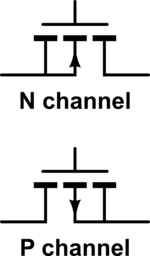
\includegraphics{mosfets.png}
\end{center}
\end{frame}

\subsection{Batteries}
\begin{frame}
\frametitle{Batteries}
Similar to capacitors batteries store electrical energy, however they store that energy via chemical reaction instead of an electric field. There are many different types of batteries. They fall into two categories; Primary, that can produce current as soon as they are made, and Secondary, that have to be charged first. There are also Dry cells and Wet cells. Common batteries are Alkaline, Li-Ion, NiCad, NiMH,ZiC, Lead-Acid. Each type has different properties, advantages and disadvantages.
\end{frame}

\part{How Radio Works}
\section{Modulations}
\begin{frame}
\frametitle{Modulation}
In radio we use different methods for ``encoding'' information on electromagnetic waves. All methods take advantage of some of the really cool parts of waves and trig.\\
Yes that math is good for something!
\end{frame}

\subsection{Continuous Wave}
\begin{frame}
\frametitle{CW}
Continuous Wave or CW communicates information by turning a signal on and off. If two parties agree on what different pasterns of On's and Off's mean then they can share information. The most common system is International Morse Code. 
\end{frame}

\begin{frame}
\frametitle{CW picture}
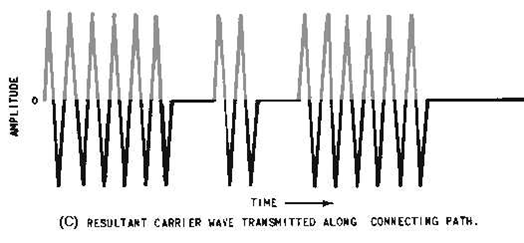
\includegraphics[height=.5\textheight]{cw.png}
\end{frame}

\subsection{Amplitude Modulation}

\begin{frame}
\frametitle{AM}
Amplitude Modulation or AM, works by keeping the frequency of a signal steady and varying the amplitude or intensity of the wave. For sounds, we simply add the sound wave to the radio wave. There are commercial AM stations, generally in lower frequencies bands. AM waves can be subject to many different forms of interference. Next to CW, AM makes for the simplest transmitters and receivers.
\end{frame}

\begin{frame}
\frametitle{AM picture}
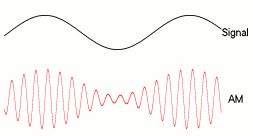
\includegraphics[height=.5\textheight]{am.png}
\end{frame}

\subsection{Single Sideband}

\begin{frame}
\frametitle{SSB }
\begin{columns}
\column{.4\textwidth}
AM is really easy but isn't very efficient. The image to the right shows the power of an AM wave. The center spike is the Carrier, and holds no useful information. The smaller peaks on either side are mirrored across the carrier. If we remove everything but on of the sides we can more efficiently use power and bandwidth. This is called Single Side band
\column{.6\textwidth}
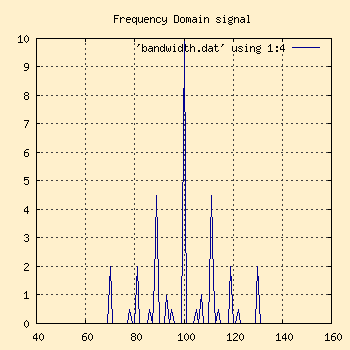
\includegraphics[width=\textwidth]{amfft.png}
\end{columns}
\end{frame}

\begin{frame}
\frametitle{SSB Continued}
From the graph we can see there are two different sidebands, one on either side of the carrier. The one that is higher in frequency is the ``Upper'' Sideband and the lower one is the ``Lower'' Sideband. For historical reasons we Upper Sideband (USB) on frequencies higher than 10MHz, and Lower Sideband on frequencies lower than 10MHz. There are also times when we use Vestigial Sideband, that is one and a part sidebands, namely for sending images.
\end{frame}

\subsection{Frequency Modulation}

\begin{frame}
\frametitle{FM}
FM or frequency modulation works by varying the frequency of the signal to encode information. FM takes the most bandwidth in that you have clear enough room on either side of the center frequency to allow for a fully modulated signal.
\end{frame}

\begin{frame}
\frametitle{FM Picture}
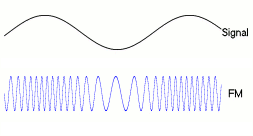
\includegraphics[height=.5\textheight]{fm.png}
\end{frame}

\subsection{Phase Modulation}

\begin{frame}
\frametitle{Phase Modulation}
Related to FM is Phase Modulation. Instead of changing the frequency, we adjust the phase of a signal. The same circuits that process FM can handle PM.
\end{frame}

\subsection{Extra layers}
\begin{frame}
\frametitle{AFSK, Packet, etc.}
We can add layers on top of these simple modulation systems to encode information. AFSK Audio Frequency Shift Keying, is a digital mode that encodes 0's and 1's as audio tones that can be sent using one of the modulations. Packet radio is a particular protocol for sending information, generally using AFSK. APRS is a way of formatting data send via packet to report the position and other information that can show up on a map.
\end{frame}

\begin{frame}
\frametitle{APRS}
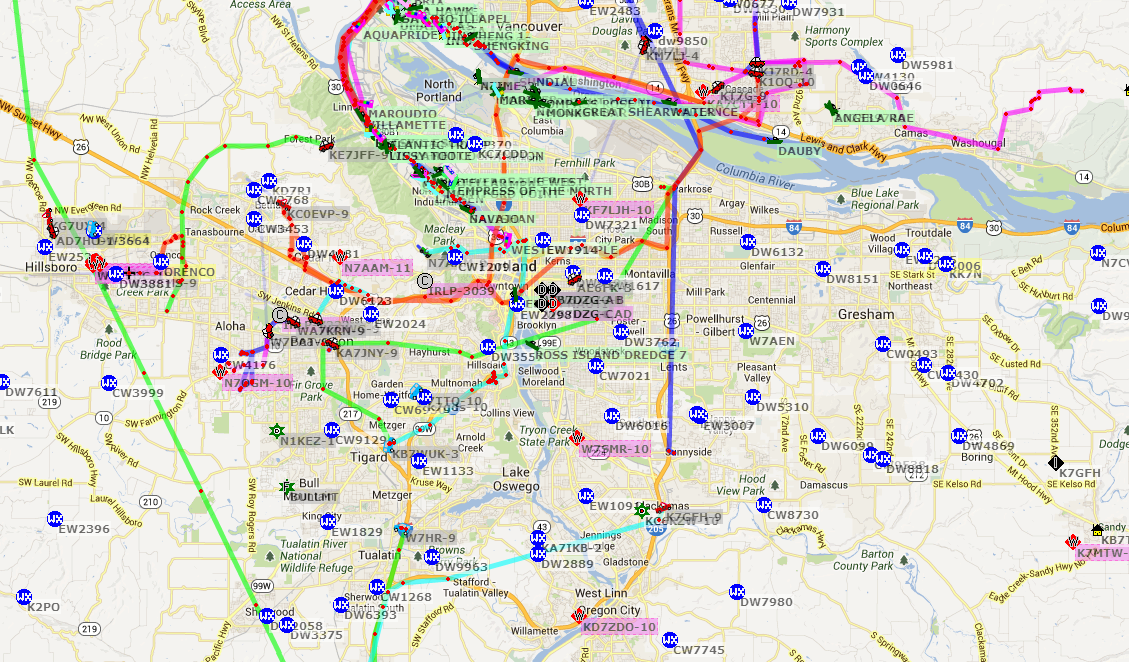
\includegraphics[width=.9\textwidth]{aprspdx.png}
\end{frame}
\section{De-Modulation}

\begin{frame}
\frametitle{De-Modulation}
De-Modulation is the process of extracting information from a radio wave. All receivers are built from the same basic components. The antenna feeds an RF amplifier, A mixer and local-oscillator steps the frequency down to something easier to process, an intermediate frequency (IF). An IF amplifier feeds the de-modulation stage which then into an audio amplifier and out to a speaker. 
\\
It is important to remember that these devices are made of circuits built from the components from the previous section.
\end{frame}

\begin{frame}
\frametitle{Simple Radio}
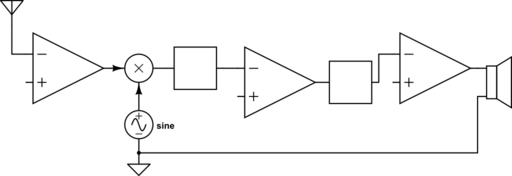
\includegraphics[width=.9\textwidth]{simplereciever.png}
\end{frame}

\subsection{AM}
\begin{frame}
\frametitle{The detector}
The AM demodulation device is called a Detector. Essentially it removes the carrier from the signal and leaves only the information, which for the most part is audio.
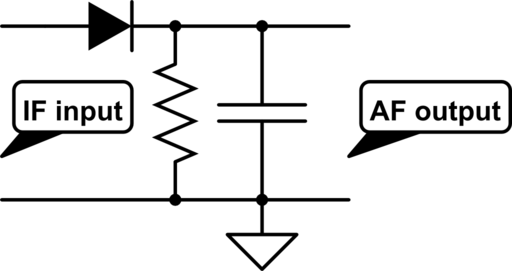
\includegraphics[width=.9\textwidth]{simpledetector.png}
\end{frame}

\subsection{SSB}

\begin{frame}
\frametitle{SSB}
As a SSB signal is just an AM signal without the carrier, it is simple enough to replace it and use the same Detector. An extra component called a Beat Frequency Oscillator is used to replace the carrier that is removed from when transmitting.
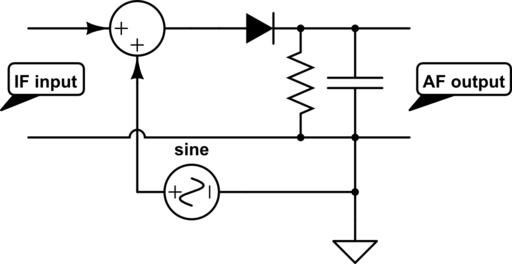
\includegraphics[width=.9\textwidth]{simpleproductdetector.png}
\end{frame}

\subsection{FM}
\begin{frame}
\frametitle{FM}
By far the most complex demodulation circuit is the discriminator used with FM signals. For the purpose of the test you only need to know the type of circuit, not how to build one. 
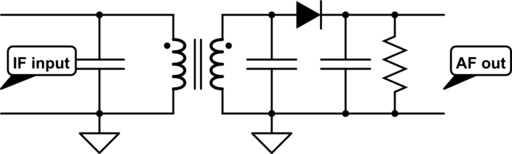
\includegraphics[width=.9\textwidth]{simplediscriminator.png}
\end{frame}

\section{The Transceiver}
\begin{frame}
\frametitle{Modulation and De-modulation together}
For the sake of space it is worth while to combine a transmitter and receiver.
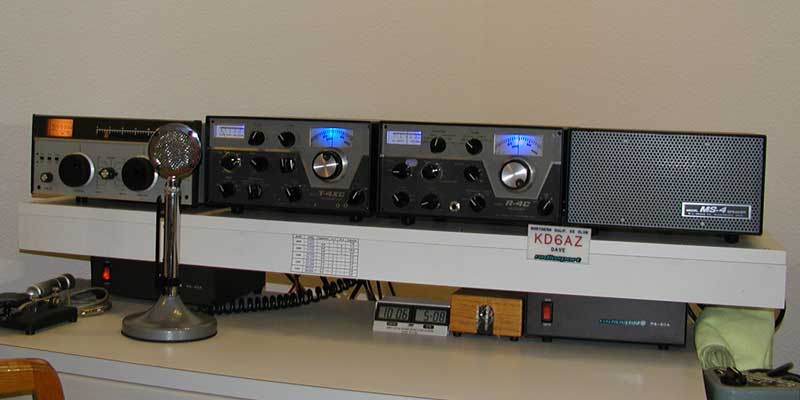
\includegraphics[height=.6\textheight]{drake4.jpg}
\end{frame}

\begin{frame}
\frametitle{Basic}
The simple looking idea is to just hook both a receiver and transmitter to the same antenna, like so.
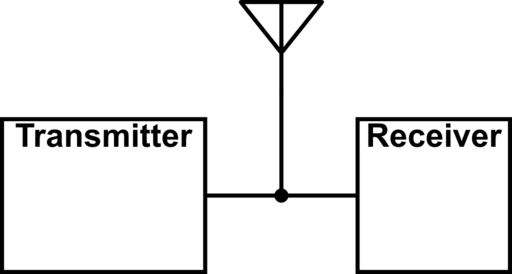
\includegraphics[height=.5\textheight]{simpletr.png}
\end{frame}

\begin{frame}
\frametitle{Real}
The problem with the simple setup is that the energy from the transmitter goes right into the receiver. Remember all those amplifiers in the receiver, they will amplify the very strong signal and then the magic smoke that makes everything work will get out. So \ldots
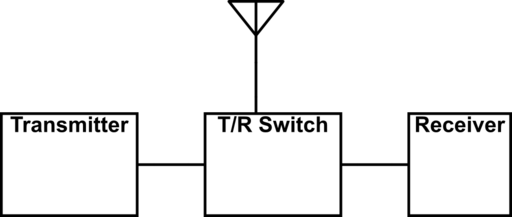
\includegraphics[width=.8\textwidth]{simpletrworks.png}
\end{frame}

\begin{frame}
\frametitle{TR Switch}
The Transmit Receive switch very quickly disconnects either the transmitter or the receiver so that the reliever doesn't blow up.
\end{frame}

\section{Repeaters}

\begin{frame}
\frametitle{Repeaters}
A repeater is just a radio that transmits what it hears. They are generally placed on high places where they can see large areas. They use a technique called Duplex, where it simultaneously receives and transmits on different frequencies. Radios automatically switch between the ``input'' and ``output'' frequencies so you don't have to. We often refer to repeaters by their output frequency, and sometimes by their callsign.
\end{frame}

\subsection{Offset}

\begin{frame}
\frametitle{Offset}
The difference between the input, the frequency the repeater listens to, and the output, the frequency the repeater transmits on, is called the offset. The standard offset is part of the band plan. The direction of the offset is also part of the band plan.\\

\begin{tabular}{|l|r|}
\hline
2m & 600 KHz\\ \hline
1.25m & 1.5MHz \\ \hline
70cm & 5MHz \\
\hline
\end{tabular}

\end{frame}

\begin{frame}
\frametitle{Offset Examples}
A couple of sample offsets on 2 meters are.\\
147.16MHz uses a standard positive offset, has an input of 147.76MHz.\\
146.78MHz again with a standard but negative offset has an input of 146.18MHz.\\
It can be difficult to remember if one part of a band is positive or negative so we often write frequency as 147.16+ or 146.78-
\end{frame}

\subsection{Tones}

\begin{frame}
\frametitle{Tones}
Because there is a limited number of locations that are good to place repeaters lots of them end up at the same place. If we don't do anything one can easily cause another to activate. To prevent this we use special signals to make sure we only activate, these are referred to as sub-audible tones.\\

There are two types, CTCSS Continuous Tone Coded Squelch System, and DCS Digital Coded Squelch.
\end{frame}

\begin{frame}
\frametitle{Repeater Directory}
How does one find out information like offset, and tone, and other useful information about a repeater?\\
The ARRL publishes a book called the Repeater Directory.
\end{frame}

\subsection{Duplexing}

\begin{frame}
\frametitle{Duplexer's}
Unlike normal radios that don't need to transmit and receive at the same time and can use a switch repeaters inherently have to do both at the same time. The solution is called a duplexer. Duplexer's are very selective filters that allow only the transmit frequency between the transmitter and antenna, and only the receive frequency between the antenna and the receiver.
\end{frame}

\begin{frame}
\frametitle{Repeater Picture}
\begin{center}
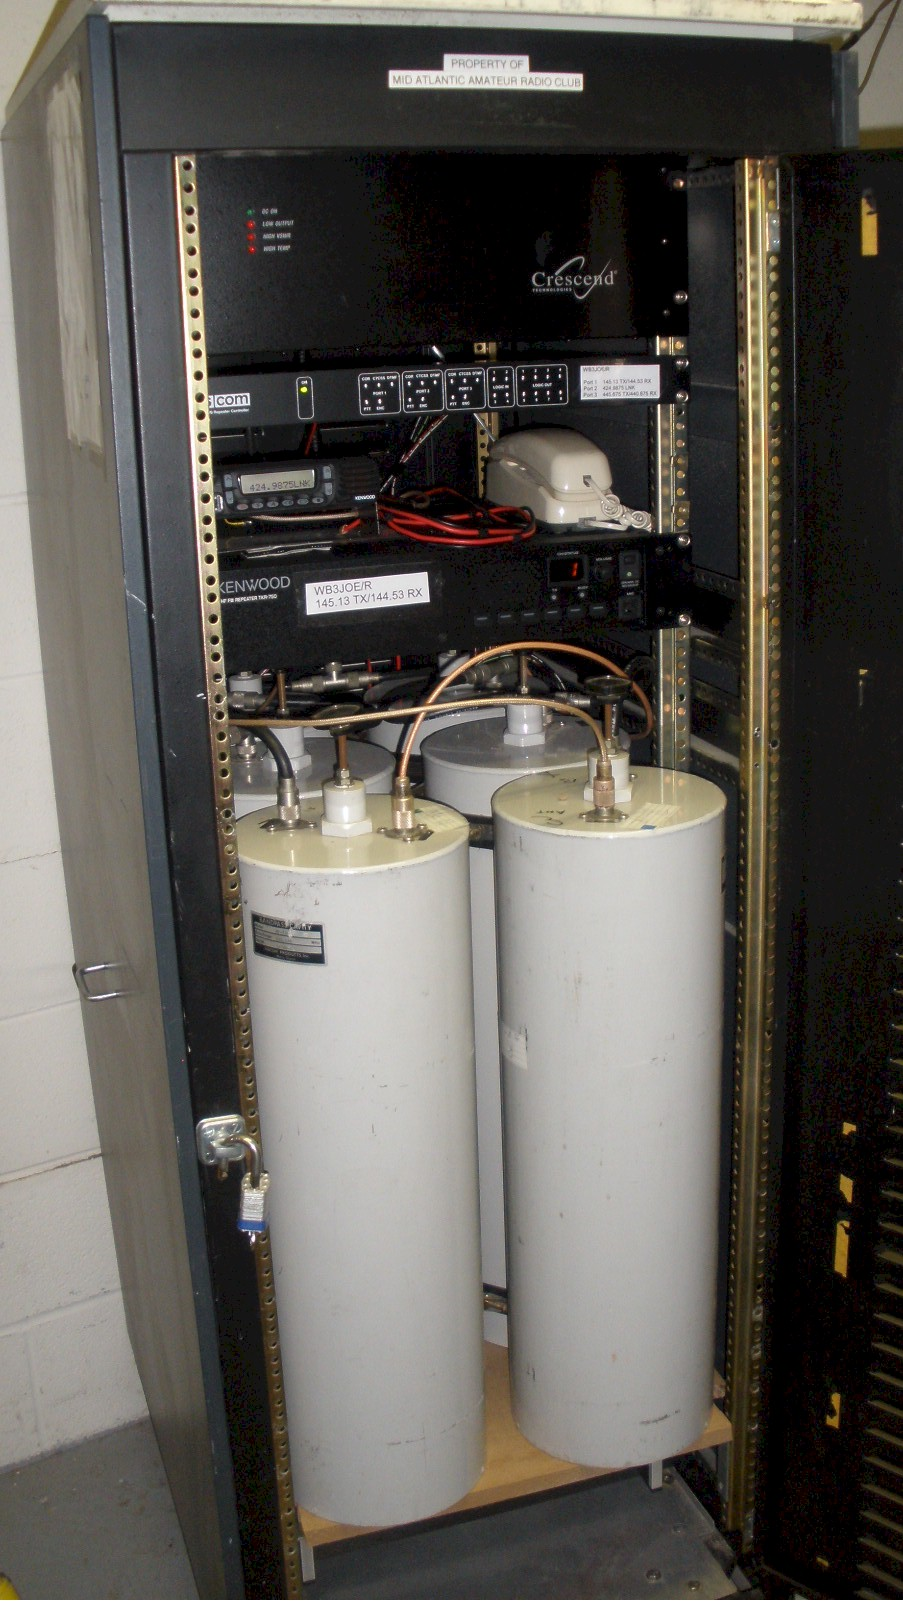
\includegraphics[height=.95\textheight]{repeater.jpg}
\end{center}
\end{frame}

\section{Satellites}

\begin{frame}
\frametitle{Satellite Duplexing}
Remember those large duplexer cans from a repeater that allow transmission and reception on the same band. Well there isn't much extra space on satellites, especially small ones for them. So how do we have satellite repeaters? Simple we separate the transmit and receive frequencies by large margins. The greater the offset the smaller the duplexer can be, when the separation is large enough the device becomes what is known as a diplexer. A diplexer uses simple low-pass and high-pass filters to separate signals from two different bands. More practically they feed different antennas.
\end{frame}

\begin{frame}
\frametitle{Satellite Duplexing}
The convention for describing which bands a satellite operates on uses one or two letters. If there is one letter then the satellite only beacons on that band, if there are two letters the satellite receives on the first letter and transmits on the second. Band letters are H for HF, V for VHF, U for UHF, L for L-band, K for K-band.  Most satellites use mode V/U, meaning they listen on VHF (2-meters) and transmit on UHF (70-cm).
\end{frame}

\subsection{Doppler Shift}
\begin{frame}
\frametitle{Doppler Shift}
Satellites are moving really, really fast, on the order of miles per second. At this speed as they move overhead we have to contend with the Doppler shift, the apparent change in frequency of a wave of emitted by a moving object. As the satellite approaches the frequency increases, and as it moves away the frequency decreases. This is just like a passing car. The hard part with satellites is the shift you see, is the same shift it sees from you, meaning while you have to tune ``up'' to hear it when listening, you have to tune ``down'' so it can hear you.
\end{frame}

\subsection{Tracking}
\begin{frame}
\frametitle{Satellite Tracking}
In order to keep track of where satellites are, we use specially formatted numbers called orbital elements. These describe certain aspects of the where a satellite is at. Given these numbers, your location, and the time you can calculate exactly where a satellite is at.
\begin{center}
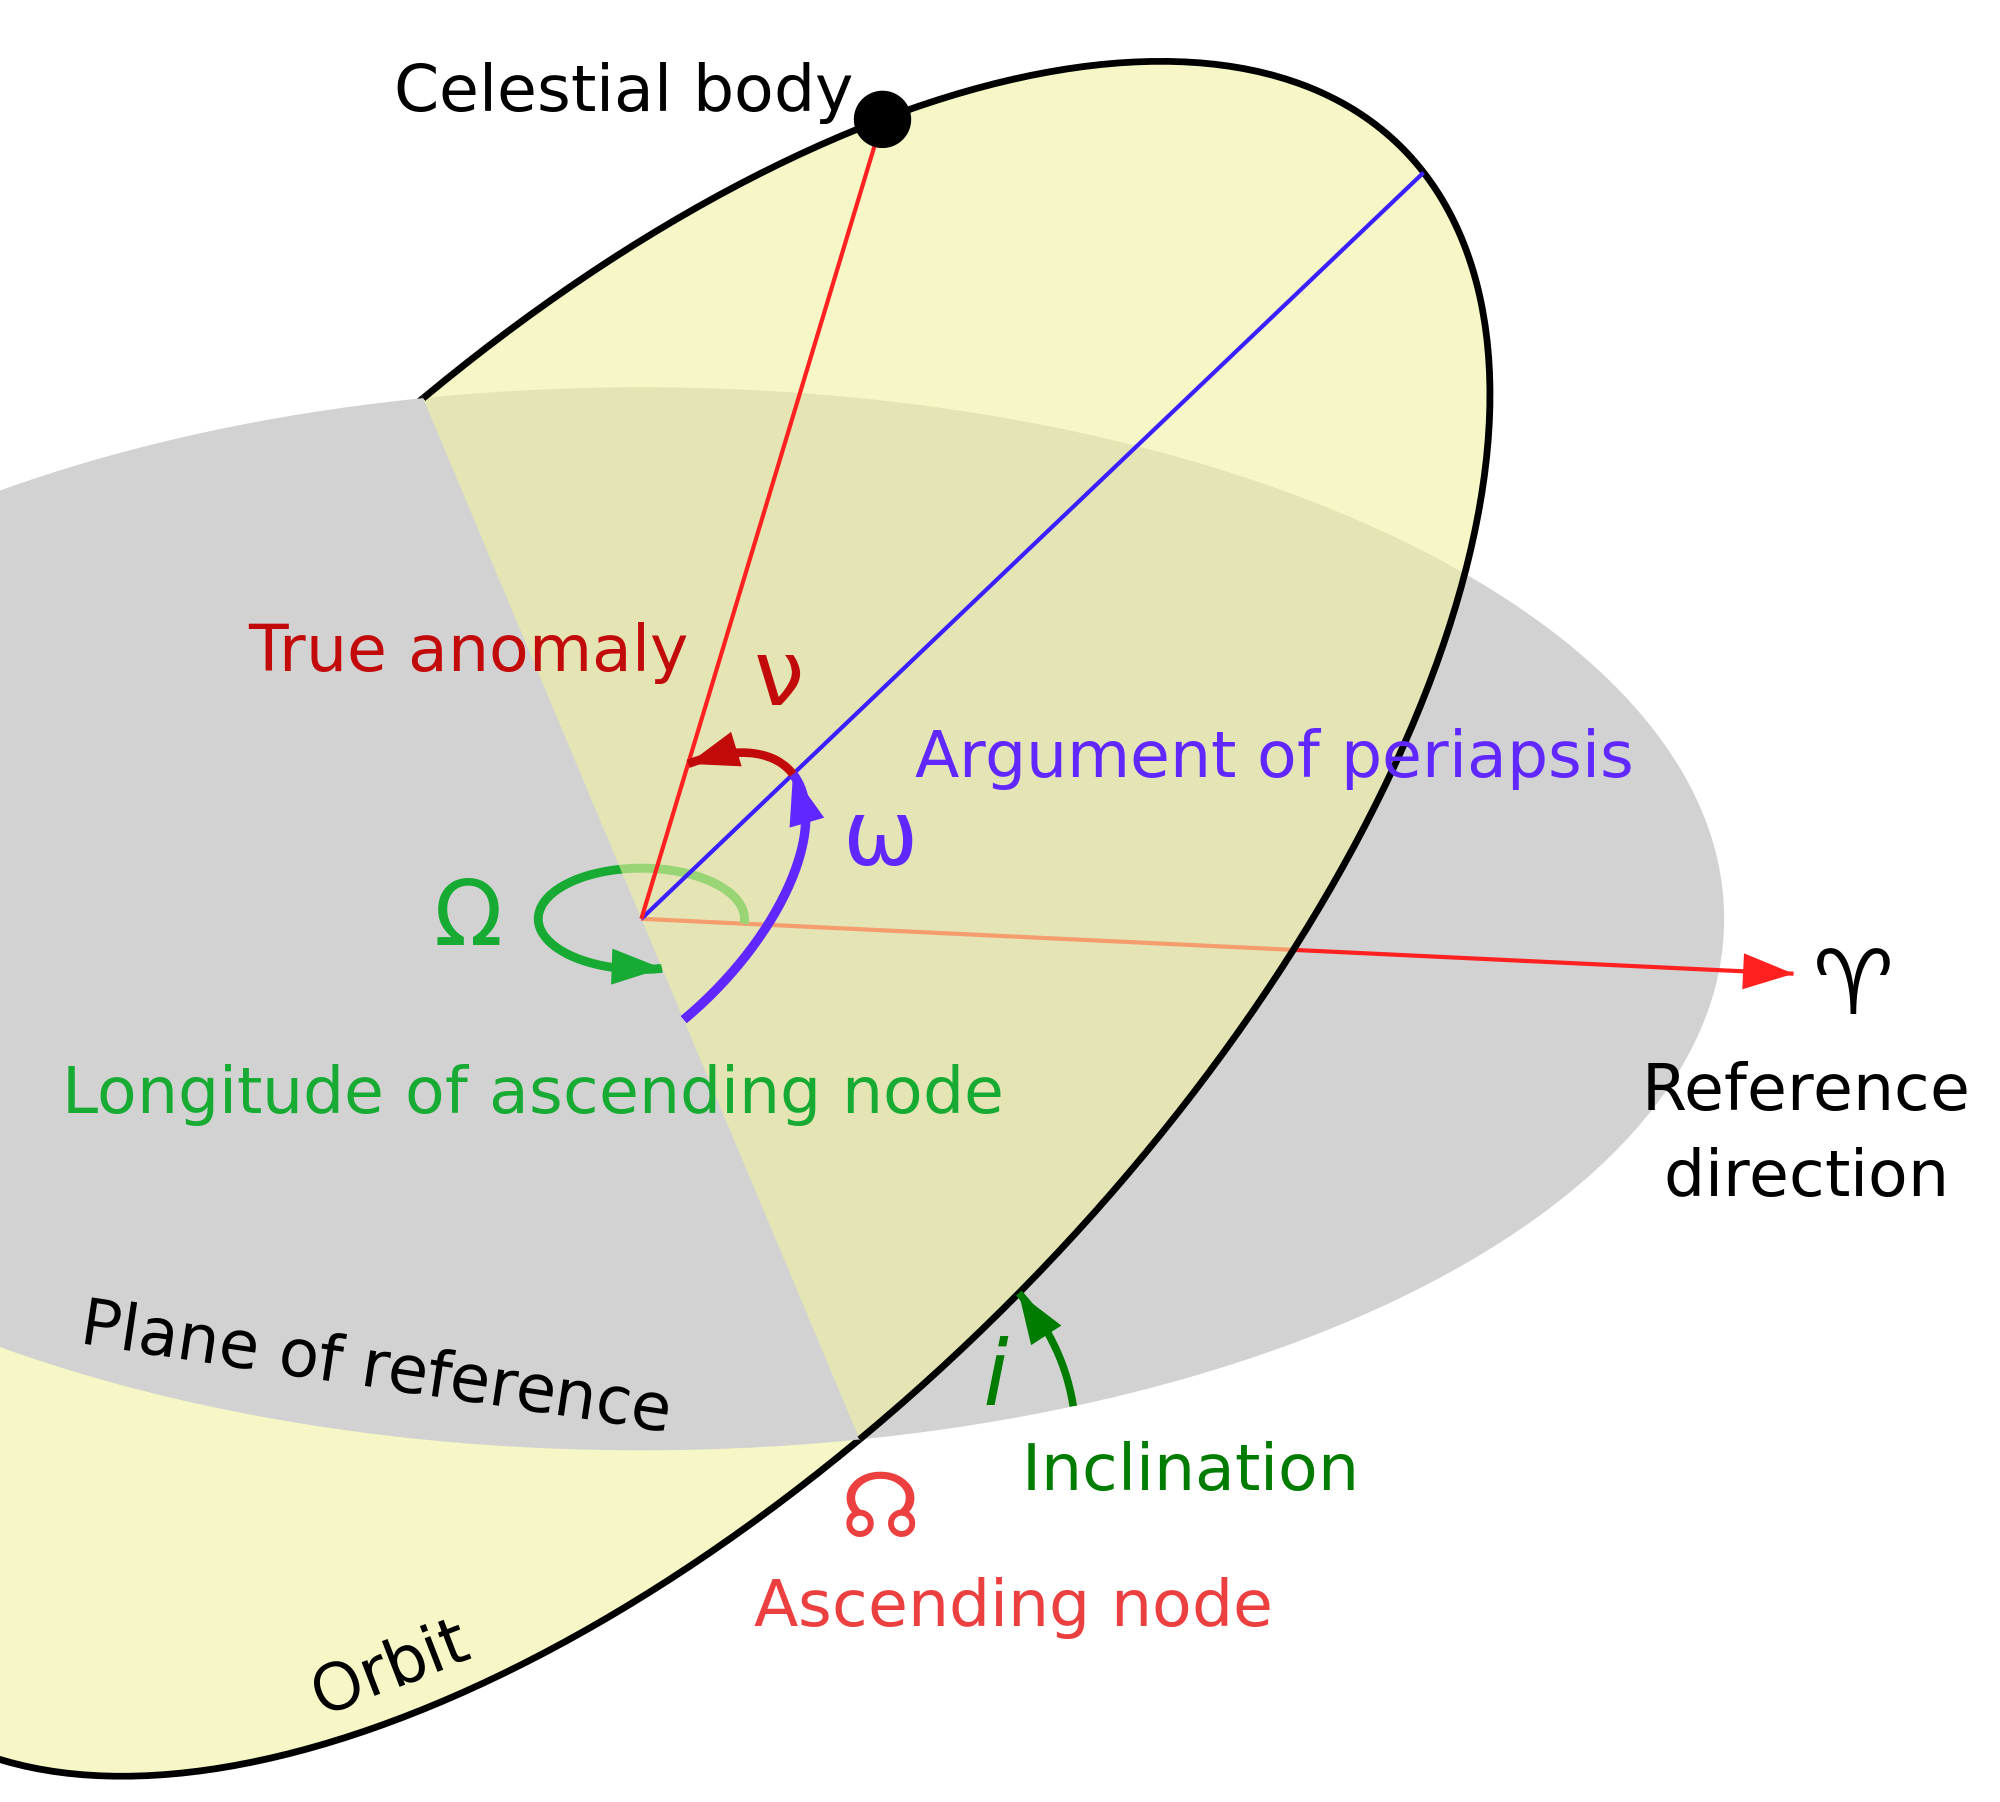
\includegraphics[height=.5\textheight]{orbitelements.png}
\end{center}
\end{frame}

\section{Digital Modes}
\begin{frame}
\frametitle{Its a digital World}
There are many digital modes out there, some encode digital data into digital signals.\\
Some encode analog signals into digital signals.
\end{frame}

\begin{frame}
\frametitle{Baud}
In the digital world there are two important rates.\\
The first is the Baud rate or number of symbols sent per second. In this case a symbol can be a particular tone, or even a change in phase or amplitude.\\
The second is the bit rate, to calculate the bit rate you take the number of bits per symbol and multiply it by the baud rate.\\
Often the bit rate and baud rate are the same, but not always. Some techniques such as Phase Shift Keying can support many bits per symbol.
\end{frame}

\subsection{Digital Voice}
\begin{frame}
\frametitle{Digital Voice}
There are several digital modes that allow analog voice to be sent using digital signals. These are APCO Project 25 (p25), D-STAR, and AOR ARD9800. These all work similarly to cellphones and VoIP.
\end{frame}

\subsection{RTTY}
\begin{frame}
\frametitle{RTTY}
RTTY - Radio TeleTYpe, is the original digital mode. It is slow 50 to 300 baud, or bits per second, that is a single text message in 4-25 seconds. It uses Frequency Shift Keying (FSK) and transmits two tones one for a ``high'' or 1, and a different one for a ``low'' or 0. RTTY machines have long been used by military and diplomatic posts, using encryption methods RTTY allows for slow, but reliable communications.
\end{frame}

\subsection{Packet}
\begin{frame}
\frametitle{Packet}
Packet radio uses AFSK generally sent using FM on VHF and above, and SSB on HF. In packet the baud rate is the bit rate. On HF speeds of a whopping 300 baud, and on VHF and up speeds range from the common 1200 baud and the extreme 9600 baud. This translates into 1.2-9.6Kbps, or about 0.5-4.3 MegaBytes per hour, or one seventy-fifth the speed required to stream netflix on the lowest quality setting.
\end{frame}

\begin{frame}
\frametitle{Packet modems}
To use things like packet you need something to MODulate, and to DEModulate signals. Put them together and we get a modem. Many devices add features for controlling things like.\\
\begin{itemize}
\item Mailbox(es)
\item BBS
\item DigiPeaters
\item Addressing
\item Error correction
\end{itemize}
Together we call this a Terminal Node Controller or TNC.
\end{frame}

\begin{frame}
\frametitle{Packet Networks}
Packet networks are configured much like how the internet works, just much smaller. ``Users'' connect to nodes, these nodes can connect to each other. If there are enough nodes lined up, messages can move over great distances. At times it is possible for messages to move across the country and even the world entirely by bouncing from radio to radio.
\end{frame}

\begin{frame}
\frametitle{The Internet}
There are message handling systems that combine the scale and speed of the internet and the robustness of radio. One such system is Winlink 2000 (yes people still use things like 2000 in names). Nodes in the system decide try to move messages through the internet, and if not over radio, special servers track messages to ensure they get delivered to the appropriate user.
\end{frame}

\subsection{APRS}
\begin{frame}
\frametitle{APRS}
The Automatic Position Reporting System APRS (pronounced A-pers) encodes position data in standard packet formats. Other information such as weather, messages, even icons. The system has ``Igates'' or internet gateways that pass information to internet servers. \hyperlink{www.findu.com}{findu.com} and \hyperlink{www.aprs.fi}{aprs.fi}
\end{frame}

\section{Linked Repeaters}

\begin{frame}
\frametitle{Linked Repeaters}
Some repeaters are linked using radios, one such system is the Peak Radio Association system. This network allows users all over the state and parts of Washington and California to speak to each other. It does take a second or two for all the links to activate.
\end{frame}

\begin{frame}
\frametitle{IRLP and EchoLink}
The Internet Repeater Linking Project or IRLP connects repeaters using the internet, audio from one repeater are sent to others. You can access a specific repeater by using the apropriate DTMF tones on your radio.\\
Echolink allows users to connect radios, computers, phones, tablets, etc\. to their network. The result is similar to IRLP though you don't have to have a radio to use echolink. Popular echolink nodes can atract radio operators from all over the world.
\end{frame}

\part{Antennas and Feedline}

\section{Antennas}
\begin{frame}
\frametitle{Antennas}
Any radio amateur will tell you that while a million watts is cool, at the end of the day its the antenna that does the real work.\\
Antennas take radio signals in the form of electrons moving in wires and converts that signal into electromagnetic waves, and back.\\
Improperly antenna configurations can even damage your radio! A 5 watt radio with a great antenna can get a lot more work done than 1000 watt radio with a poor antenna.
\end{frame}

\subsection{1/4 Vertical}
\begin{frame}
\frametitle{Quarter Wave Vertical}
\begin{columns}
\begin{column}{.6\textwidth}
Probably the simplest antenna to look at is the 1/4 vertical. It is made of two parts, a vertical section of wire that is 1/4 the wavelength long, and ground.\\
The wavelength is that of the wave in the wire, which is not the same as in free space. Fortunately the math has already been done for us, over and over and the equation is: $L\left(ft\right) = \frac{234}{F \left(MHz\right)}$
\end{column}
\begin{column}{.4\textwidth}
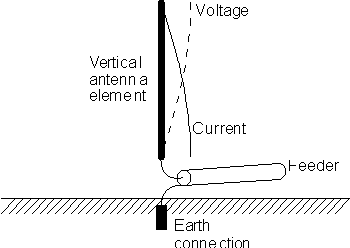
\includegraphics[width=\textwidth]{qwavevert.png}
\end{column}
\end{columns}
\end{frame}

\begin{frame}
\frametitle{Grounding}
\begin{columns}
\begin{column}{.5\textwidth}
The problem with this is that the antenna needs to be close to ground, but we want antennas to be really high up so they can ``see'' further.\\
The solution is to create a ``fake'' ground that can elevated with the vertical section.
\end{column}
\begin{column}{.5\textwidth}
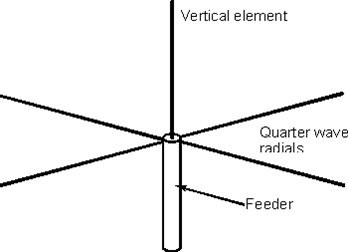
\includegraphics[width=\textwidth]{qwavevertwground.png}
\end{column}
\end{columns}
\end{frame}

\begin{frame}
\frametitle{Vertical Radiation Patern}
The vertical radiates well in all horizontal directions, but doesn't do very well up or down.
\begin{center}
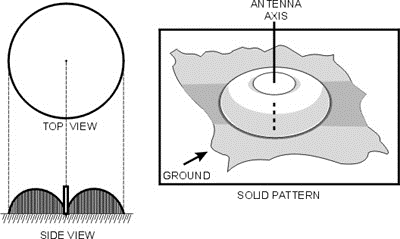
\includegraphics[height=.7\textheight]{qwavevertrad.png}
\end{center}
\end{frame}

\subsection{1/2 Wave Dipole}

\begin{frame}
\frametitle{1/2 Wave Dipole}
Another common antenna is the 1/2 wave dipole. This is made by placing two 1/4 wave wires in lines and feeding them in the middle. This uses one of the wires as the ``ground''. The total length is twice that found for the 1/4 vertical.
\begin{center}
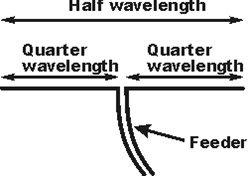
\includegraphics[height=.5\textheight]{hwavedipole.png}
\end{center}
\end{frame}

\begin{frame}
\frametitle{Dipole Radiation patern}
The dipole radiates well perpendicular to the length of the wire. A dipole running north-south will radiate east-west.
\begin{center}
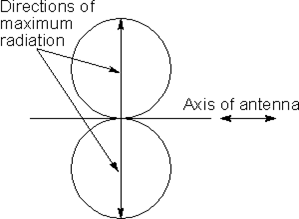
\includegraphics[height=.5\textheight]{hwavedipolerad.png}
\end{center}
\end{frame}

\subsection{Gain}
\begin{frame}
\frametitle{Gain}
\begin{columns}
\begin{column}{.5\textwidth}
The yellow dot and line are the antennas. The red circle is the radiation pattern of the vertical, and the green circles are the pattern for the dipole. The distance from the center indicates the strength.\\
Notice how the dipole is better in two directions but worse the other two. The apparent increase in signal strength when the dipole is ``pointed'' in the right direction is called Gain.
\end{column}
\begin{column}{.5\textwidth}
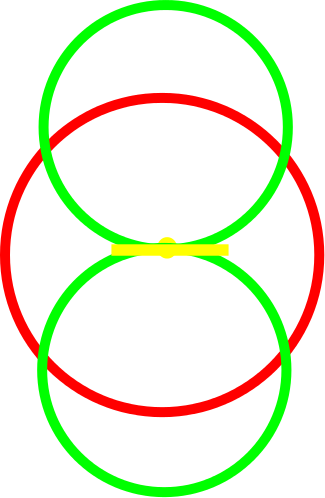
\includegraphics[width=\textwidth]{vertvsdipole.png}
\end{column}
\end{columns}
\end{frame}

\begin{frame}
\frametitle{dB's}
We generally measure Gain in terms of decibels, dB. This is a ratio measurement, meaning it compares two things. We often will compare antennas to an ``isotropic'' antenna or a perfect 1/2 wave dipole, dBi and dBd. If an antenna claims some gain without saying what it is compared to ASK!. for POWER the equation is $dB=10\log\frac{P}{P_0}$ and for voltage its $dB=20\log\frac{V}{V_0}$ where P and V are your apparent signal and $P_0$ and $V_0$ are the starting points.\\
A good rule to remember is that a change of 3dB in power is a change of a factor of 2 for power, and a change of 6dB is a factor of 2 for voltage. We almost always talk in terms of power.
\end{frame}

\subsection{The Yagi}
\begin{frame}
\frametitle{The Yagi-Uda}
If we add another length of wire behind the dipole to reflect incoming signals into the antenna, and more in front to direct signals we get a Yagi-Uda, or Yagi.\\
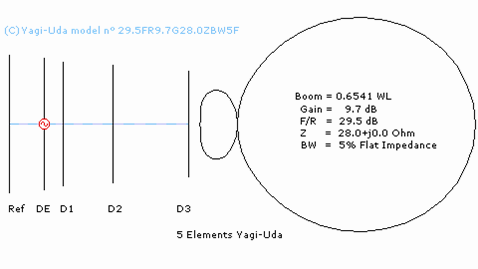
\includegraphics[height=.5\textheight]{yagi.png}
\end{frame}

\begin{frame}
\frametitle{Giant Antennas}
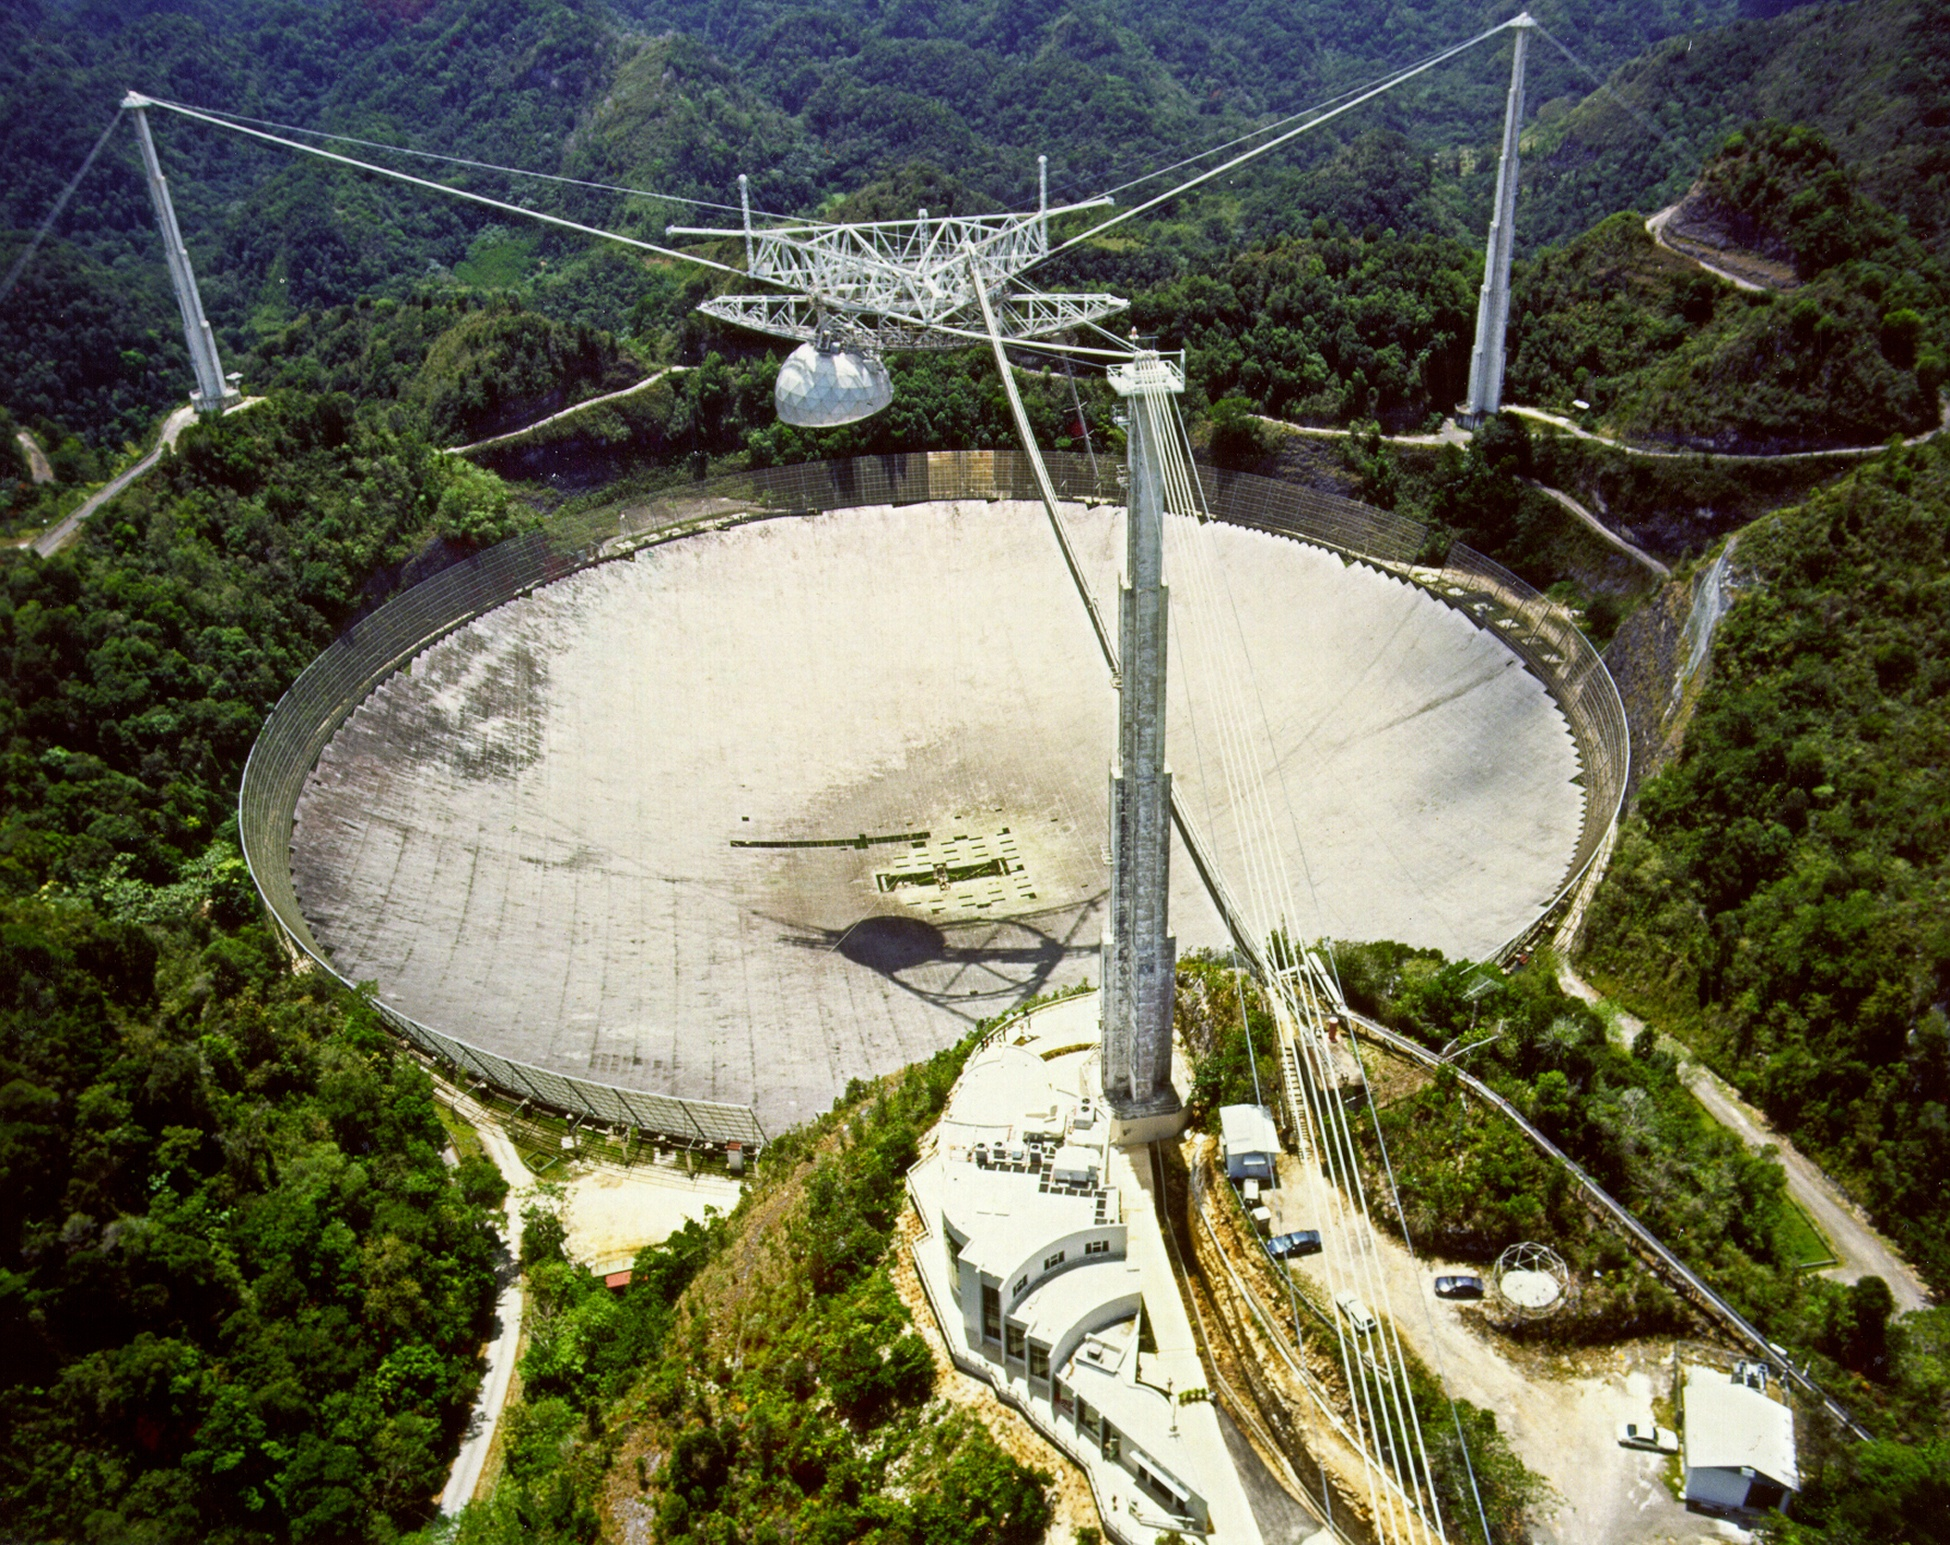
\includegraphics[width=.49\textwidth]{arecibo.jpg}
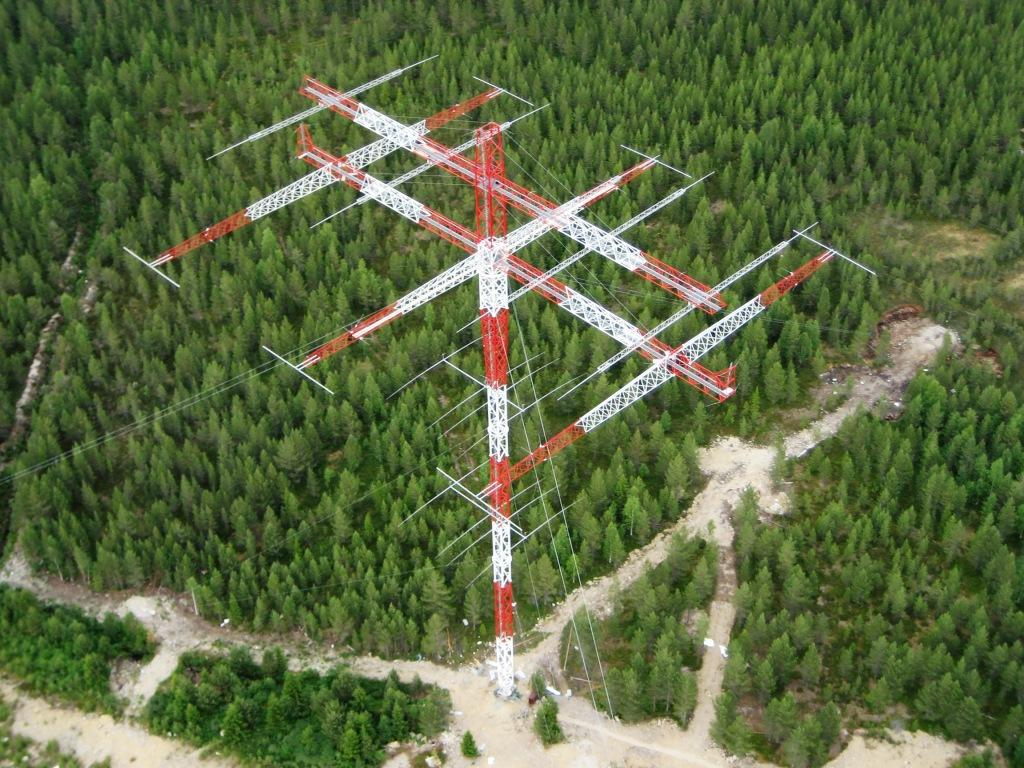
\includegraphics[width=.49\textwidth]{160myagi.jpg}
\end{frame}

\section{Feedline}
\begin{frame}
\frametitle{Feed Me!}
Antennas need a connection to the radio. We call this connection ``feedline''. It has one job, carry the signal between the radio and antenna as efficiently as possible.
\end{frame}

\subsection{Waveguide}
\begin{frame}
\frametitle{Wave Guide}
One type of feedline is the waveguide, which is really just a hollow tube in which a signal bounces off the walls as it moves from end to end. Fiber optic cables are an example of a waveguide for light. In the waveguide the signal moves as a radio wave. The size of the guide depends on the wavelength of the wave, they are almost never used below UHF as they get really really big. 
\end{frame}

\subsection{Coaxial Cable}
\begin{frame}
\frametitle{Coax}
By far the most common feedline in use is Coaxial Cable. They are made of a center wire surrounded by an insulator, which is in turn surrounded by a metal shield and another outer insulator. More layers of shields and insulators can be added as needed. The term Coaxial refers to the fact that all the components share a common axis.
\end{frame}

\begin{frame}
\frametitle{More Coax}
Coax has several advantages over other feedlines. It is generally flexible and the metal shield and outer insulator allows it to go almost anywhere, even underground. However it is important to watch out for kinks, damage to the insulation and water.\\
Once water gets into the cable it is done for, it corrodes the metal components, and changes the properties of the cable.
\end{frame}

\begin{frame}
\frametitle{Hardline}
One type of coax is called hardline, it is not flexible. It is very low loss, can be pressurized to keep water out, and is less affected by water in the first place.\\
However it is hard to work with, it requires special equipment, its is heavy and very expensive.\\
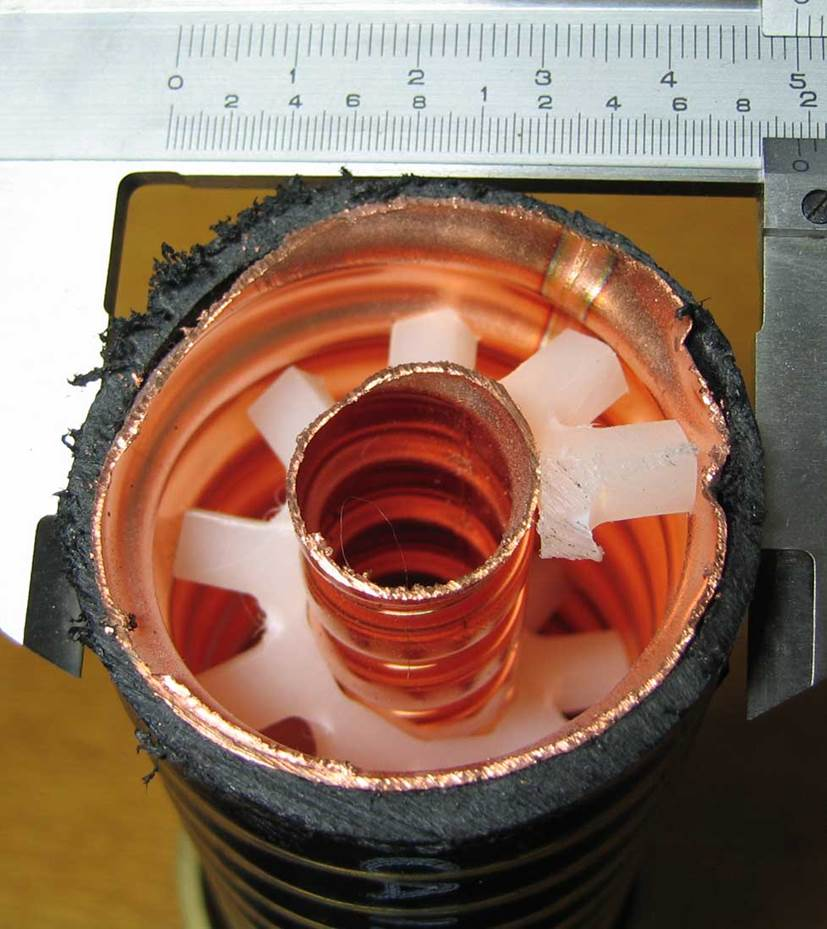
\includegraphics[height=.4\textheight]{4inhardline.jpg}
\end{frame}

\begin{frame}
\frametitle{Losses}
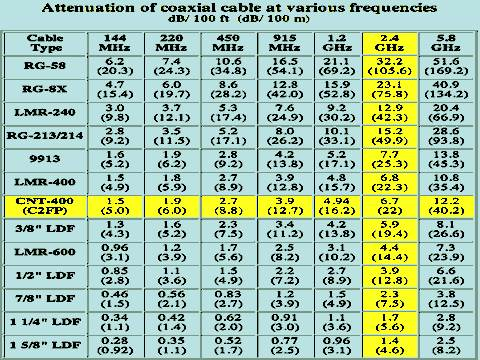
\includegraphics[height=.9\textheight]{coaxatten.jpg}
\end{frame}

\section{Impedance}
\begin{frame}
\frametitle{Impedance}
Impedance is the opposition to the flow of current in an AC circuit (e.g.\ RF). It is a combined measure of the ohmic resistance, capacitance, and inductance of a circuit. Antennas have an impedance, feedlines are designed to have a known impedance, and radios have input and output impedance.\\
Common impedance measurements in amateur radio are 50$\Omega$ and 300$\Omega$, while TV cables are normally 75$\Omega$ 
\end{frame}

\begin{frame}
\frametitle{Impedance Matching}
If there is a mismatch in impedance then power will reflect from the point of the mismatch. This is bad! signals from the antenna bounce back to the antenna and don't reach the radio. Even more dire strong signals from the radio don't make it to the antenna and bounce back into the radio!\\
The most efficient systems match impedance as closely as possible.
\end{frame}

\subsection{SWR}

\begin{frame}
\frametitle{The SWR meter}
A simple tool for checking impedance matches is the SWR meter, they simply show you the ratio of power going out to power coming back. A match of 1:1 is perfect, most things will work with a mismatch of up to 2:1, any higher and there is a real problem.
\end{frame}

\begin{frame}
\frametitle{Check everything first}
So a good SWR means all is good right? \pause Well not exactly\ldots \\\pause
Lets say you have a 50W radio and a broken antenna with really lossy cable say 10.6dB.\\
When it reaches the antenna and reflects back it is down to 4.3W and radio only sees 0.4W.\\
$SWR=\frac{F+R}{F-R}=\frac{50.4}{49.6}=1.01:1$\\
This is a great SWR but all the power is going into the cable. The radio will be happy but you have just made your feedline a 50W heater.
\end{frame}

\begin{frame}
\frametitle{SWR Problems}
So how do you deal with SWR problems?\\
\begin{enumerate}
\item Adjust the impedance of feedline and antennas to minimize the extent of the mismatch and reduce the SWR.
\item Use an antenna tuner that doesn't fix the mismatch, but will protect the radio from reflected power by making it look like there is a match.
\end{enumerate}
\end{frame}

\begin{frame}
\frametitle{Antenna Tuners}
Antenna tuners work by changing the apparent electrical properties of a system by adding inductance or capacitance thus are able to match the impedance between two components at a single point. The two places tuners are commonly found are right at the output of the transmitter (some radios even have built in tuners), and at the base of the antenna. Tuners at the radio protect if from reflected power, tuners at antennas maximize the power that gets radiated.
\end{frame}

\begin{frame}
\frametitle{Tuner Pictures}
\begin{columns}
\begin{column}{.5\textwidth}
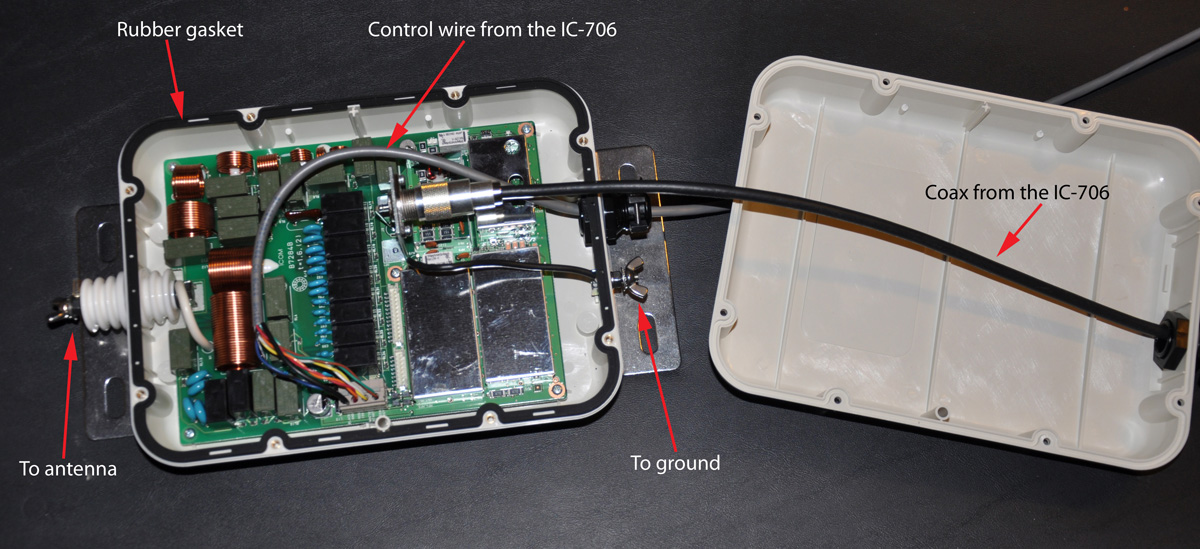
\includegraphics[width=\textwidth]{ah4inside.jpg}
\end{column}
\begin{column}{.5\textwidth}
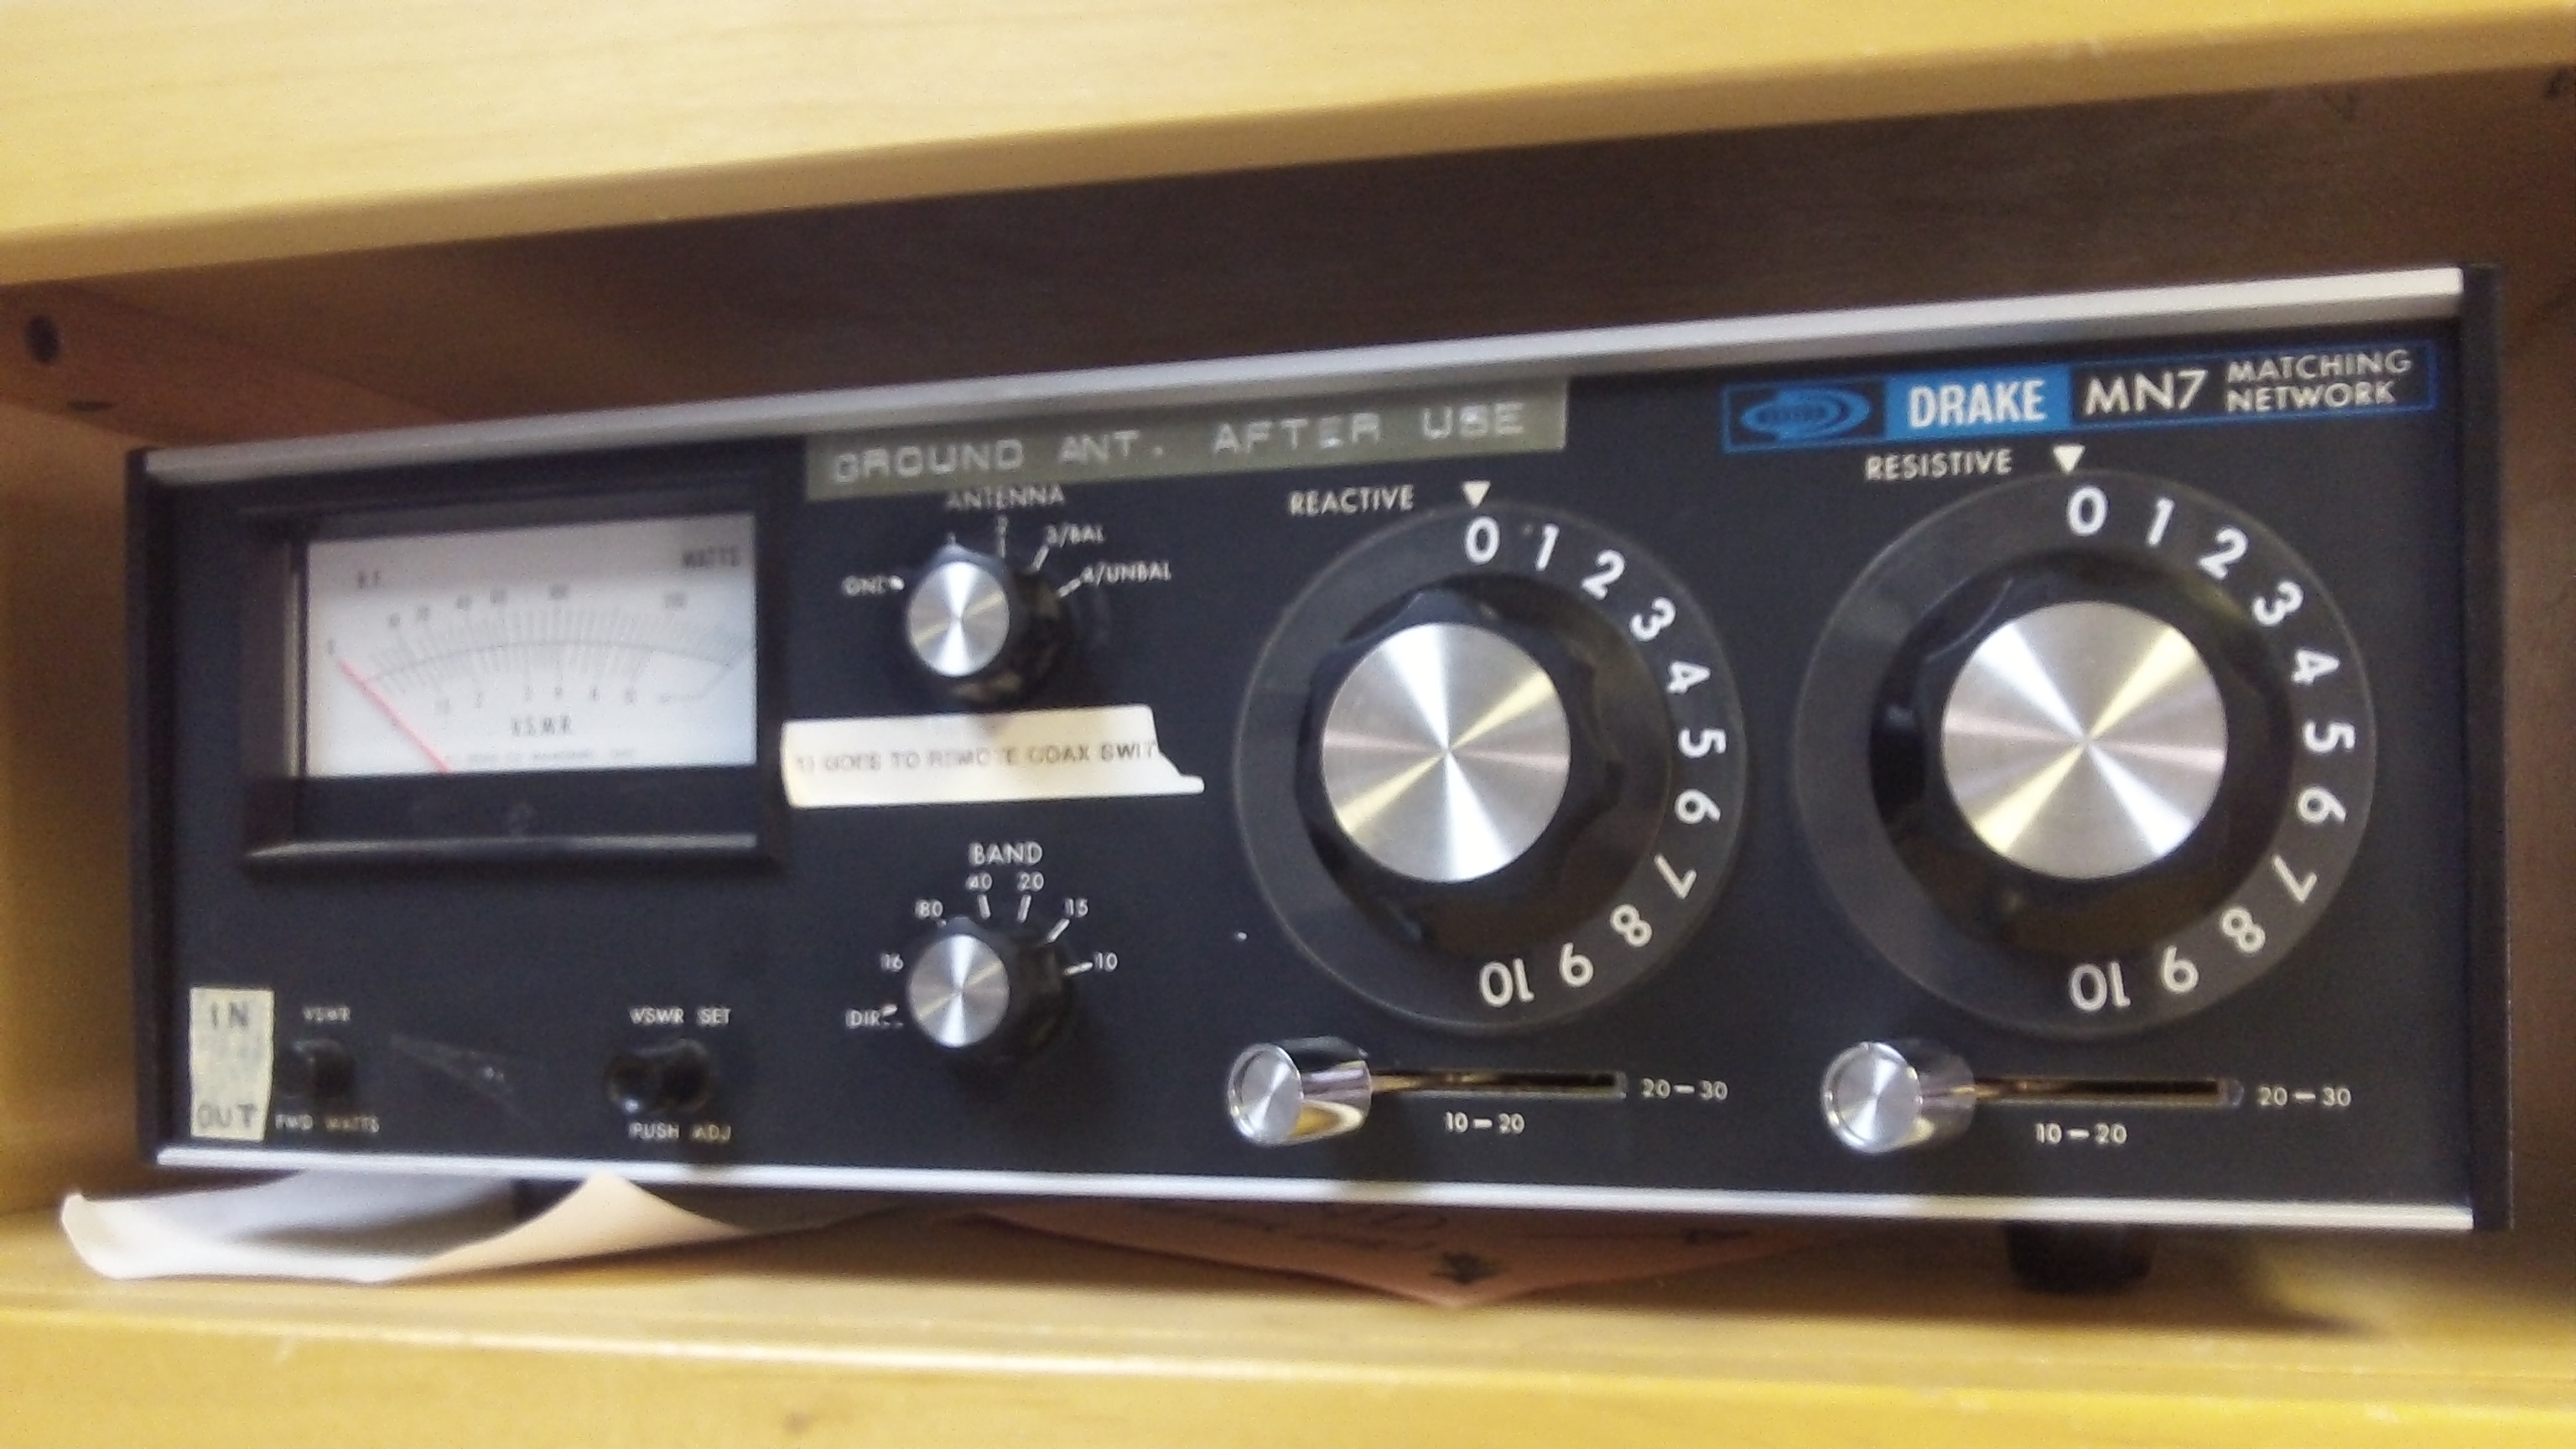
\includegraphics[width=\textwidth]{drakemn7tuner.jpg}
\end{column}
\end{columns}
\end{frame}

\begin{frame}
\frametitle{Dummy Load}
Sometimes you want to test your equipment without actually transmitting over the air. In this case you need something that has an impedance match, and will be able to safely dissipate the RF energy. Enter the Dummy load, a device made to do just that. Be sure to always check the ratings for power and duty cycle.\\
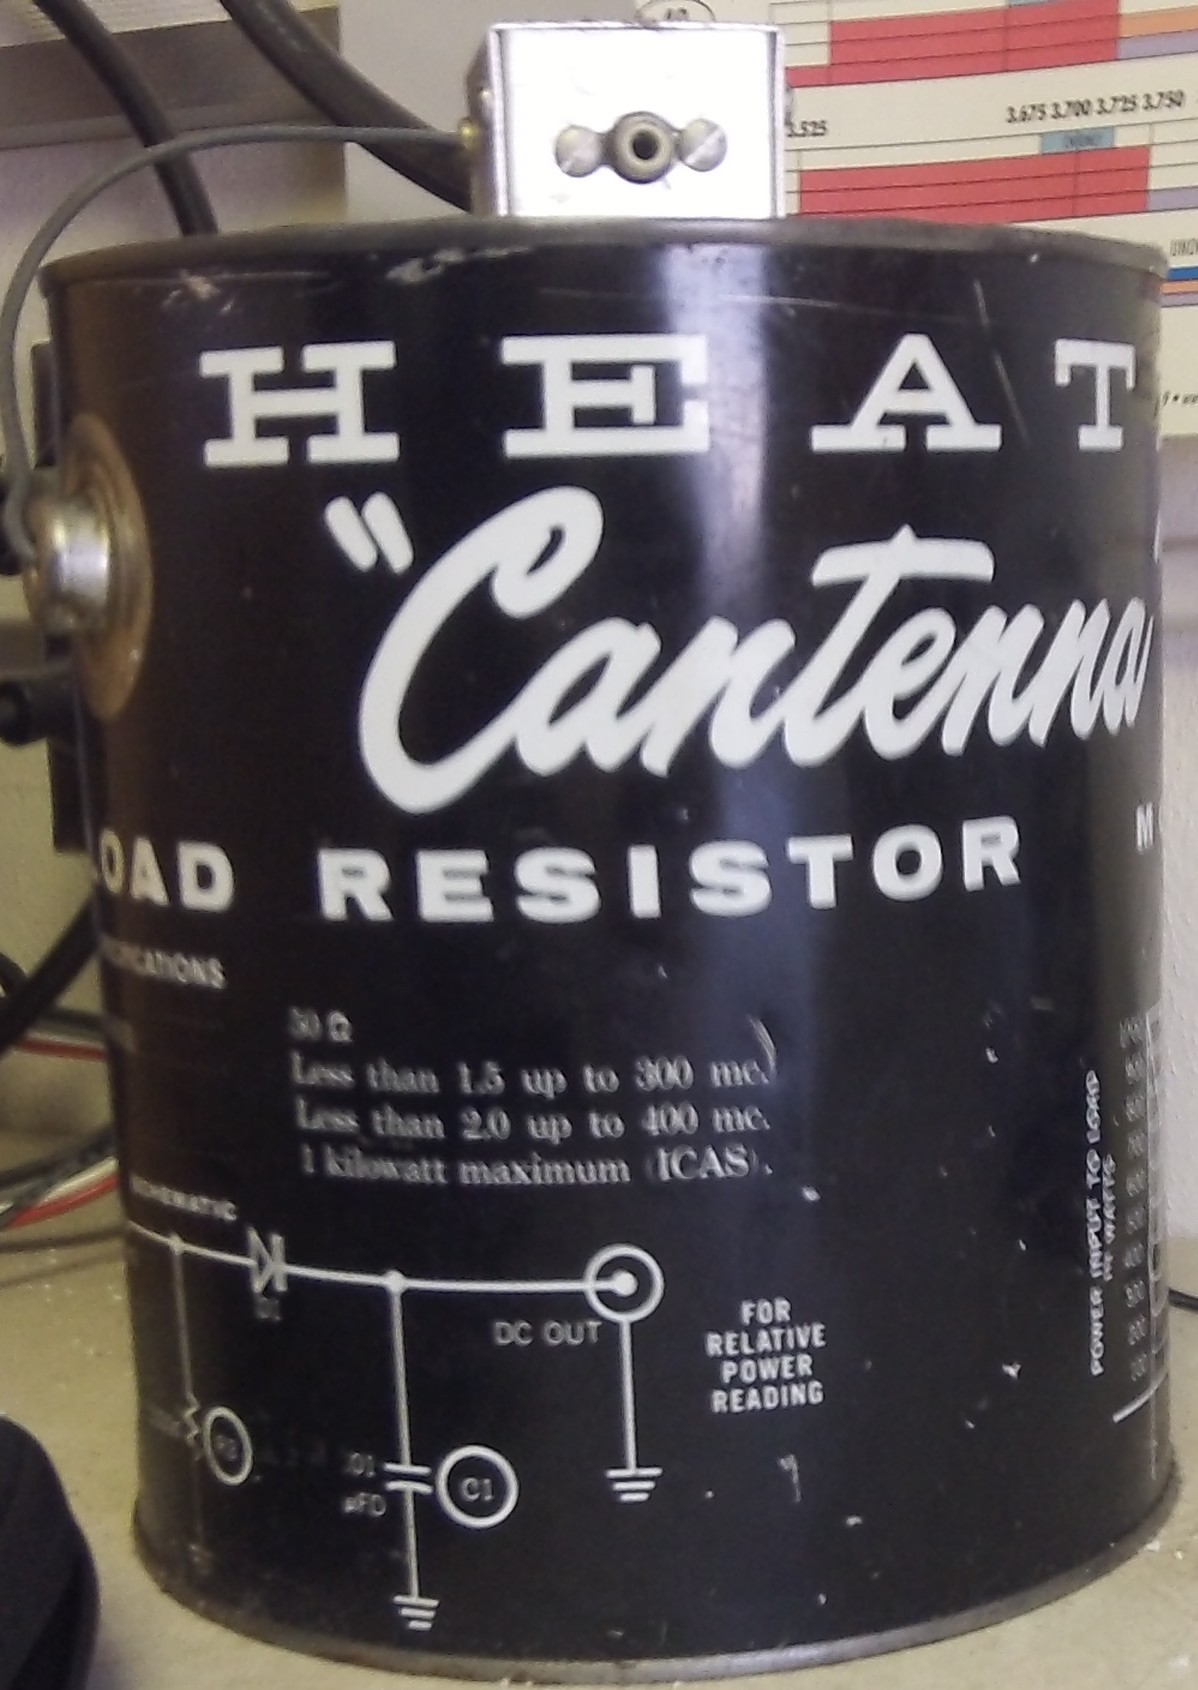
\includegraphics[height=.5\textheight]{heathcantenna.jpg}
\end{frame}

\section{Connections}
\begin{frame}
\frametitle{Connections}
So now we have feedlines, radios, and antennas, how do we actually connect them? There are four common RF connectors.\pause\\
The PL-259(SO-239) Are by far the most common and work well on HF, ok on VHF and not so good on UHF and above, they also can handle relatively large amounts of power. They are sometimes called UHF connectors even though they aren't very good for UHF. \pause \\
The Type N connector can't handle quite as much power as the 259 (though still high enough for amateur use), but works better at higher frequencies (through SHF) and is much more weather resistant. They are also much more expensive than the 259. \pause \\
The BNC or Bayonet Neil-Concelman work well up to about 2GHz, at lower power levels. The ``Bayonet'' part makes them easy to connect/disconnect \pause \\
The SMA or Sub Miniature is to the BNC what the N is to the 259, better performance into SHF, but lower power.

\end{frame}

\begin{frame}
\frametitle{Connectors continued}
259's and N's are common for ``Base'' or ``Mobile'' stations, namely in cases where you are not likely to disconnect and reconnect cables often. In ``Hostile'' weather environments it is not common to protect these connections from water.\\
BNC's and SMA's are common on handheld radios. While the spec's say they are safe up to several thousand watts it isn't advised to run more than 50-ish on either. BNC's are also prone to tarnish and this changes the properties of the connector. They do not handle outdoors well for any length of time, though a threaded version TNC is an option.
\end{frame}

\part{Power and Safety}
\section{Shock}
\begin{frame}
\frametitle{Shock!}
Electricity is the number one cause of electrocution in the US!\\
You may have heard that its the voltage that hurts and the current that kills. While true remember that $V=IR$ and if V goes up I probably is as well.\\
Less than 100mA can disrupt your heart, and it can take only 30V on your skin to reach 100mA across the heart.
Besides heart problems current creates heat that can cause serious burns.
\end{frame}

\begin{frame}
\frametitle{Shock Prevention}
Some ways to mitigate shock danger are.\\
\begin{itemize}
\item Turn off and disconnect equipment before working on it.
\item Remember to discharge capacitors.
\item Don't circumvent safety features such as power interlocks.
\item If you can't power down something then:
\begin{itemize}
\item Use one hand, keep the other in your pocket
\item Take of rings, watches, and anything else metal
\item Remember things happen faster than you can react, one wrong move and you could be dead before you know it.
\end{itemize}
\end{itemize}
\end{frame}


\begin{frame}
\frametitle{Fuses}
Fuses are your friend.\\
Fuses are designed to open a circuit when overloaded, they burn so you and your equipment don't.\\
Always be sure to use the proper fuse, they are rated for voltage, current, and slow/fast burn
\end{frame}

\begin{frame}
\frametitle{Fuse Picture}
\includegraphics[width=\textwidth]{fuse.jpg}
\end{frame}

\section{Grounding}
\begin{frame}
\frametitle{House wiring}
The current standard code for electrical wiring in the US calls for 3-prong outlets. The three prongs are Hot, Common, and Ground. The hot supplies the current, the common provides a return route, and the ground acts as a safety. In the breaker box the common and ground are supposed to be bonded together.
\end{frame}

\begin{frame}
\frametitle{House picture}
\includegraphics[height=.9\textheight, width=.9\textwidth]{outletground.jpg}
\end{frame}

\begin{frame}
\frametitle{GFCI}
In some cases a Ground Fault Circuit Interrupter may be required by code. These devices open the circuit if there is a current imbalance between the hot and common lines. They look like normally outlets with two buttons on them. These provide an extra level of protection especially in locations such as outdoors or bathrooms. Though be aware that some devices may not function properly when connected to GFCI protected circuits, namely devices with their own GFCI installed.
\end{frame}

\begin{frame}
\frametitle{Radio Grounding}
Radio equipment should be properly grounded on its own. Large, clean conductors should be used running in straight lines, and as short as reasonably possible. Electrical supply stores will sell grounding bars that allow you to run short runs from devices to a common point and ground that point.
\end{frame}

\begin{frame}
\frametitle{Towers}
\includegraphics[height=.9\textheight, width=.9\textwidth]{towerground.jpg}
\end{frame}

\section{Batteries}
\begin{frame}
\frametitle{Lead Acid}
Lead acid batteries come in several different types, common in amateur use are Deep-cycle and sealed cells.\\
Typical deep-cycle batteries are rated to discharge a much larger percentage of their capacity than say a car battery. They can be charged off your car or a charger, and are relatively cheap and easy to find. However their are filled with acid that can leak if handled improperly, and can emit explosive gasses during charging.\\
Sealed cells are more expensive and harder to find, but are much more resistant to mishandling. However they can crack and leak if overcharged, overheated, or abused.\\
Both contain Lead! 
\end{frame}

\begin{frame}
\frametitle{Lithium}
Lithium batteries are becoming much more common especially in handheld radios. While most have built in circuits to prevent damage care must be taken to prevent physical abuse. Overcharge, overheat, and a physical break in the container can release lithium which reacts violently with just about everything causing fire or even explosions.
\end{frame}

\section{RF Safety}
\begin{frame}
\frametitle{RF Safety}
RF energy is non-ionizing radiation, meaning it isn't capable of breaking chemical bonds. However those things that absorb it convert the RF energy into heat. RF burns can be caused without direct contact with an antenna.
\end{frame}

\begin{frame}
\frametitle{Body resonaces}
The body is resonant between 30 and 70 MHz, the head around 400MHz. The amount of absorption depends on the exact frequency, and field strength.\\
Higher power and more directional antennas create higher field strengths.
\end{frame}

\begin{frame}
\frametitle{Regs}
The FCC regulates exposure limits on all frequencies, and amateurs are included.\\
There are exemptions and special rules for stations that emit less that 50W PEP, Mobile and portable, and stations with power less than those listed in the table 1 of FCC OET Bulletin \#65.
\end{frame}

\begin{frame}
\frametitle{RF limites}
\begin{columns}
\begin{column}{.5\textwidth}
MF
\begin{itemize}
\item 160m 500W
\end{itemize}
HF
\begin{itemize}
\item 80m 500W
\item 75m 500W
\item 40m 500W
\item 30m 425W
\item 20m 225W
\item 17m 125W
\item 15m 100W
\item 12m 75W
\item 10m 50W
\end{itemize}
\end{column}
\begin{column}{.5\textwidth}
VHF All bands 50W\\
UHF
\begin{itemize}
\item 70cm 70W
\item 33cm 150W
\item 23cm 200W
\item 13cm 250W
\end{itemize}
SHF all bands 250W\\
EHF all bands 250W\\
Repeaters 500W
\end{column}
\end{columns}
Table 1. Power thresholds for routine evaluation of amateur radio stations, watts from FCC OET \#65.
\end{frame}

\begin{frame}
\frametitle{Measurement standards}
In the world of DC circuits measuring things like power and current are simple. In the world of AC (which radio is a part) it is more difficult, for one thing in DC all electrons slowly move in one direction, in AC they just kind of wiggle back and forth. The other thing is that if one uses normal calculus over a sine wave the positive and negative parts cancel each other out mathematically. We do have a few tricks up our sleeve.
\end{frame}

\begin{frame}
\frametitle{PEP, RMS, TPO}
For the AC line voltage from say a wall outlet we simplify the things by using a system called Root Mean Squared or RMS. With this we take the square root of the average of the square of the voltage, which allows you to use $P=IV$. 120V is an RMS value actual peak to peak voltage is much larger
\end{frame}

\begin{frame}
\frametitle{Measurements}
There are two areas with limits, the Controlled area in which everyone inside the area knows about the radiator and can control the radiator.\\
Uncontrolled areas are those areas where people are unaware or otherwise unable to mitigate their exposure.\\
There are three methods approved.
\begin{itemize}
\item Use field strenght equipment to measure the exposure.
\item Use antenna modeling software to predict field strengths.
\item Use the tables in OET Bulletin \#65
\end{itemize}
The last one is the easiest and most often used.
\end{frame}

\begin{frame}
\frametitle{RF mitigation}
There are several ways to mitigate exposure to RF radiation: Move the antenna, decrease antenna gain, lower power output, and change the orientation of the antenna.
\end{frame}

\section{Towers}
\begin{frame}
\frametitle{Tower Safety}
Whenever you do anything with a tower LOOK UP! Every year people are killed by not looking for power lines.\\
Always use safety gear! Falling from a tower is bad, getting hit by something/someone falling from a tower is also bad.\\
Always plan ahead, place towers such that if they fall they and everything on them will miss power lines. 10ft is the rule.\\
Use special equipment to help
\end{frame}

\part{Best Practices}

\begin{frame}
\frametitle{Common Courtesies}
Amateur radio is unique in the level of freedom, and lack of oversight we are given. We are able to get away with this because by and large we play nice with each other and with other users of radio spectrum. This has its own drawbacks, for one many ``rules'' are unwritten or just gentleman's agreements. The last bit of information isn't part of the test but should help you get on the air faster.
\end{frame}

\begin{frame}
\frametitle{Footprint}
Remember that when using phone modes that you are take up a piece of that band and that at any given time only one station can use any given piece. Anything you can do to reduce your footprint in congested bands will allow more people to use them. Turning down your power to comply with the minimal power requirement can go a long way. Using directional antennas can reduce the amount of power needed even more.
\end{frame}

\begin{frame}
\frametitle{Be Nice}
So your neighbor's TV flips out when you key up, not your problem right? Technically correct, but they also don't have to like you for it. A little bit of RFI knowhow and sincere attempt to be nice can help keep things neighborly. It never hurts to present amateur radio as a friendly and professional group of people.
\end{frame}

\begin{frame}
\frametitle{Be Patient}
Not everyone is going to be an expert operator their first day on the air. Many of us made (and still make) mistakes, and had people who helped us out. Nicely remind operators when to ID, or if the key up on top of you. Conversely remember that when a more experienced operator that them telling you to do something it is to help you out.
\end{frame}

\part{Le Fine}

\begin{frame}
\frametitle{That's it}
Questions?
\end{frame}

%
%\begin{frame}
%\frametitle{Title}
%hello world
%\end{frame}
%

\end{document}
